
\documentclass[11pt, a4paper]{article}
%\usepackage{proj1}
\usepackage{natbib}
\usepackage{fancyhdr}  
\usepackage{subcaption}
\usepackage{caption}
\usepackage{graphicx}
\usepackage{numprint}
\usepackage{multirow}
\linespread{1.25} 
\setlength{\parindent}{0cm}
\graphicspath{{Images/}}
\usepackage{hyperref}
\usepackage{amsmath}
\usepackage{amsfonts}
\usepackage{amssymb}
\usepackage{amsthm}
\usepackage{mathtools}
\usepackage{commath}
\usepackage{bbm}

%\usepackage[sc,osf]{mathpazo}
\usepackage{subcaption}
\usepackage[a4paper, top=1in, left=1.0in, right=1.0in, bottom=1in, includehead, includefoot]{geometry} %Usually have top as 1in

\usepackage{listings}
\usepackage{color} %red, green, blue, yellow, cyan, magenta, black, white
\definecolor{mygreen}{RGB}{28,172,0} % color values Red, Green, Blue
\definecolor{mylilas}{RGB}{170,55,241}


\hypersetup{colorlinks,linkcolor={black},citecolor={blue},urlcolor={black}}
\usepackage{color}
\urlstyle{same}


\theoremstyle{definition}
\newtheorem{definition}{Definition}[section]

\newcommand{\adja}{q_a}
\newcommand{\adjb}{q_b}
\newcommand{\adjaB}{q_{a,\partial \Omega}}
\newcommand{\adjbB}{q_{b,\partial \Omega}}
\newcommand{\adjB}{q_{\partial \Omega}}
\newcommand{\Adja}{\mathbf{p}}
\newcommand{\Adjb}{q}
\newcommand{\adj}{q}
\newcommand{\Adjc}{{q}_{\partial \Omega}}
\newcommand{\ra}{\rho_a}
\newcommand{\rb}{\rho_b}
\newcommand{\w}{\mathbf{w}}
\newcommand{\x}{\mathbf{x}}
\newcommand{\f}{\mathbf{f}}
\newcommand{\ve}{\mathbf{v}}
\newcommand{\n}{\mathbf{n}}
\newcommand{\h}{\mathbf{h}}
\newcommand{\K}{\mathbf{K}}
\newcommand{\hr}{\widehat \rho}
\newcommand{\jf}{\mathbf j}

\DeclareMathOperator{\sgn}{sgn}
\DeclareMathOperator{\Grad}{Grad}
\DeclareMathOperator{\Div}{Div}
\DeclareMathOperator{\Lap}{Lap}
%	\begin{figure}[h]
%		\centering
%		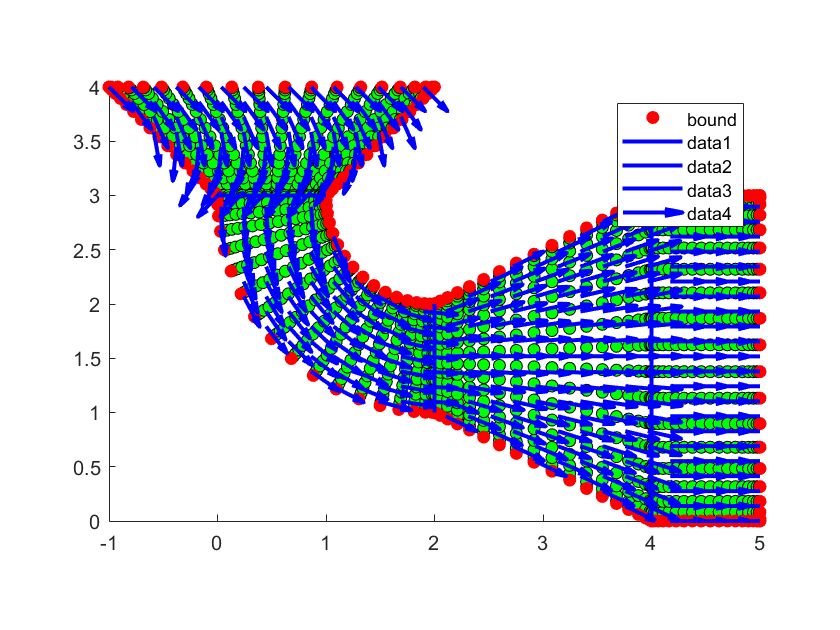
\includegraphics[scale=0.35]{F1.png}
%		\caption{Forward $\rho$ for $a = 0.01$} 
%		\label{F1}
%	\end{figure}

\begin{document}
	\section*{Paper Examples}
	\section{Neumann Source Control}
	We choose 
	\begin{align*}
		\rho_0 &= 0.25\\
		V_{ext} &= 1.5\sin(\pi x_2/5)\cos(\pi x_1/5 - \pi/5)\\
		\hr &= 0.25(1 - t) + t(0.25\sin(\pi(x_1 - 2)/2)\sin(\pi(x_2 - 2)/2) + 0.25)
	\end{align*}
	We choose the domain $[-1,1]^2$ with a time horizon $(0,1)$ and $N = 20$, $n = 11$. 
	For $\beta = 10^{-3}$, for $\kappa = -1$ we have $\mathcal J_c = 0.0018$, for $\kappa = 0$ (compared to $\mathcal J_{uc} = 0.0274$ from $\beta = 10^3$), $\mathcal J_c = 0.0017$ and for $\kappa = 1$, $\mathcal J_c = 0.0018$. Each of these computations takes around $200$ seconds for $10$ outer iterations. The results can be seen in Figures \ref{F1a}, \ref{F1b} and \ref{F1c} and the external potential acting on $\rho$ is displayed in Figure \ref{F1V}.\\
	The cost for these results is not that far from the cost with $\beta = 3$. Therefore we run the same example with $\beta = 10^{-5}$. This gives for $\kappa = -1$, $\mathcal J_c = 8.0673 \times 10^{-4}$, for $\kappa = 0$, $\mathcal J_c = 8.1989 \times 10^{-4}$, and for $\kappa = 1$, $\mathcal J_c = 8.4241 \times 10^{-4}$. Notably, these calculations only take around $20$ seconds. The results are displayed in Figures \ref{F1a5}, \ref{F1b5} and \ref{F1c5}. The controls are larger, but the difference in dynamics is smaller for different interactions.
	
	\begin{figure}[h]
		\centering
		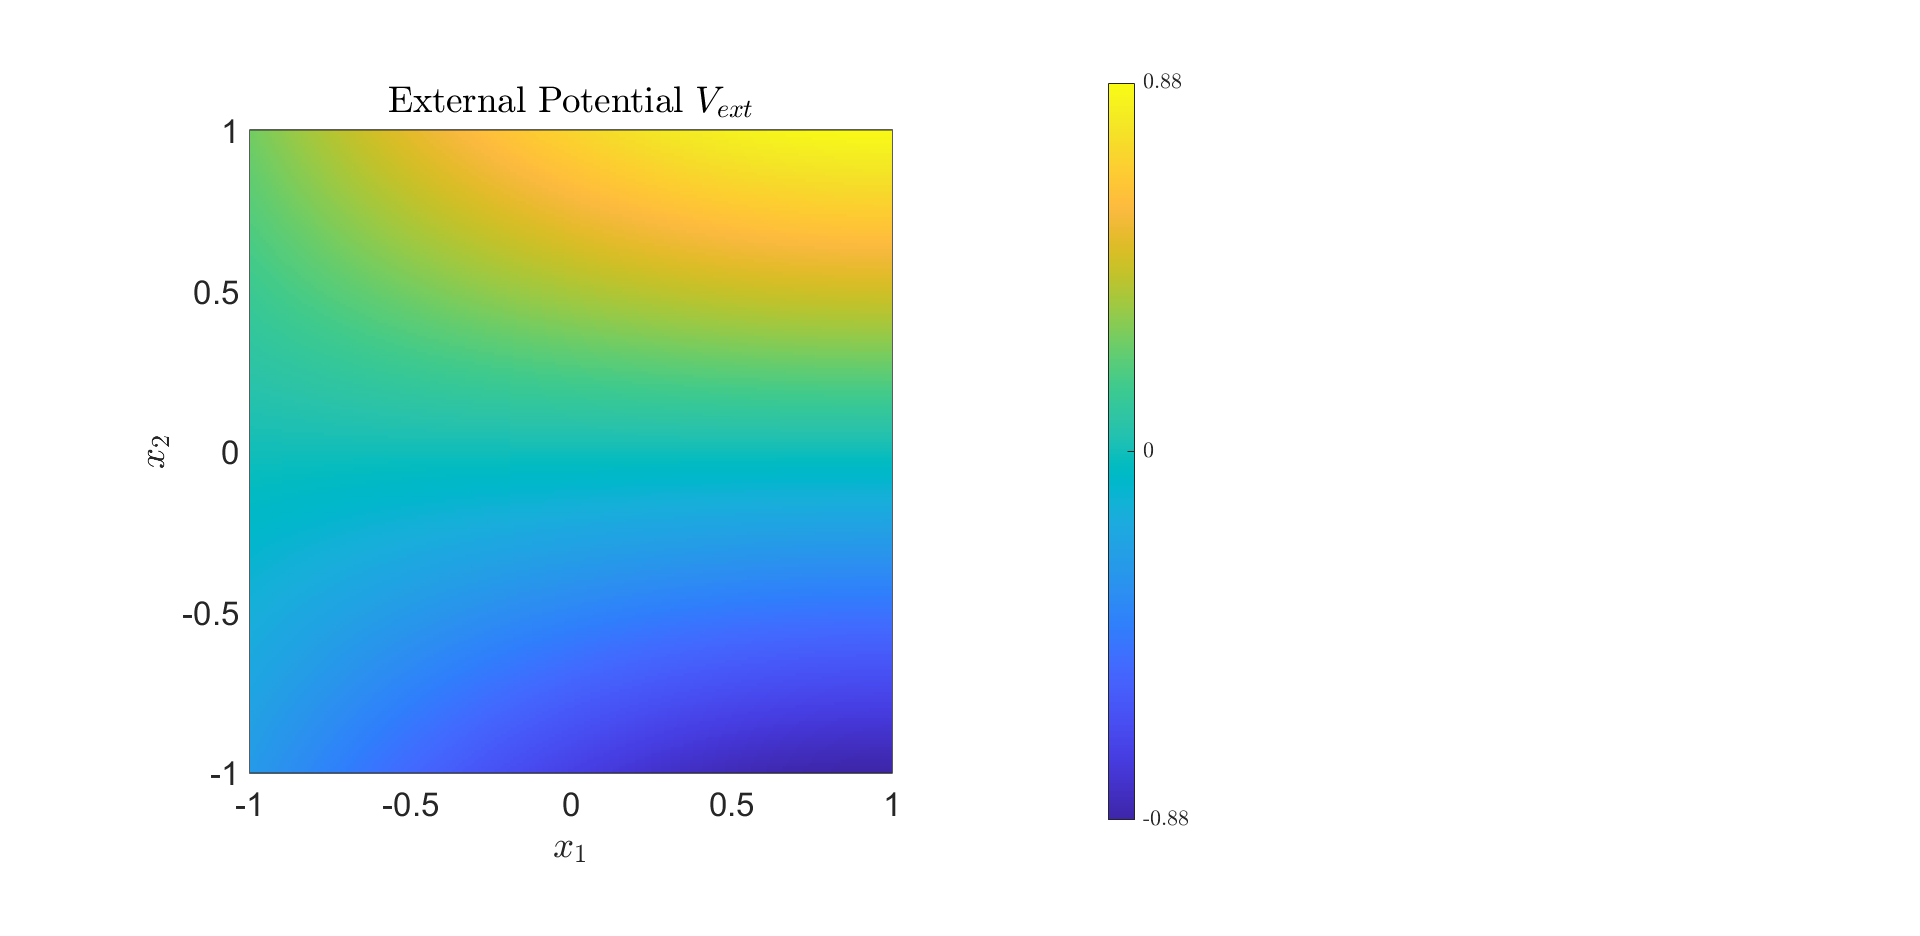
\includegraphics[scale=0.35]{SCEx1Vext.png}
		\caption{Neumann Source Control: External Potential $V_{ext}$ acting on $\rho$.} 
		\label{F1V}
	\end{figure}
	\begin{figure}[h]
		\centering
		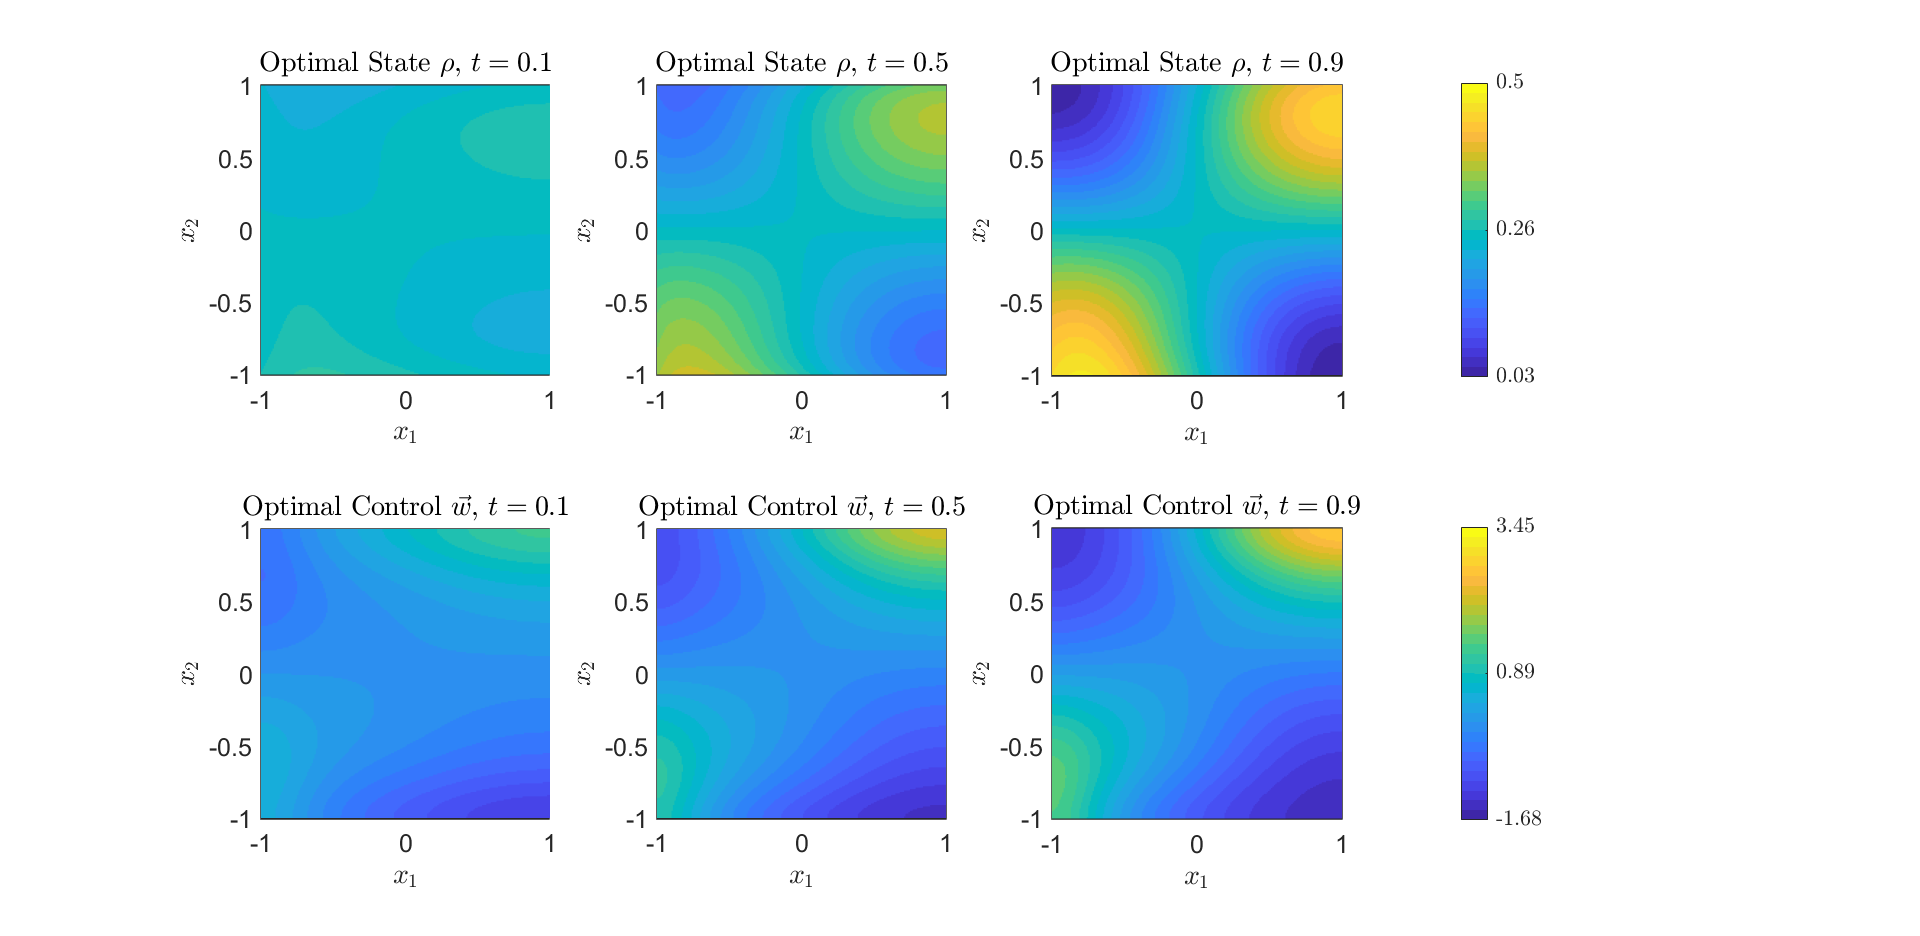
\includegraphics[scale=0.35]{SCEx1k0.png}
		\caption{Neumann Source Control: Optimal $\rho$ and optimal control for $\kappa = 0$ and $\beta = 10^{-3}$.} 
		\label{F1a}
	\end{figure}
	\begin{figure}[h]
		\centering
		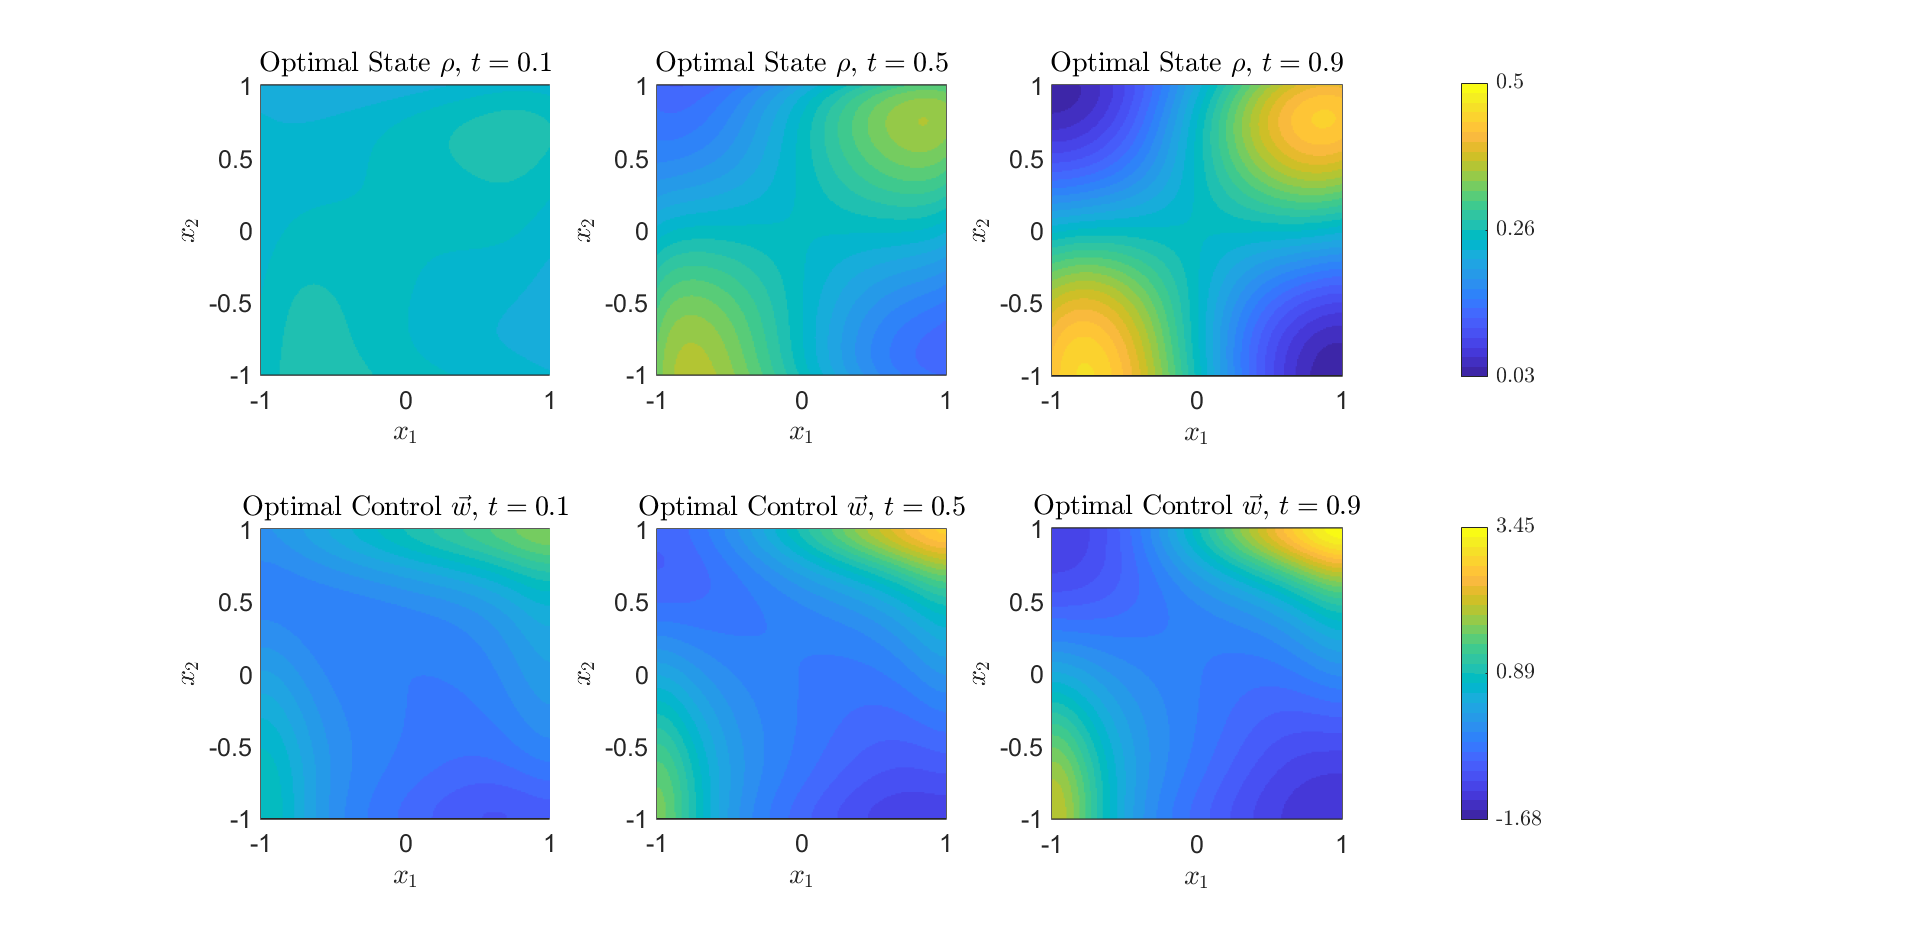
\includegraphics[scale=0.35]{SCEx1kn1.png}
		\caption{Neumann Source Control: Optimal $\rho$ and optimal control for $\kappa = -1$ and $\beta = 10^{-3}$.} 
		\label{F1b}
	\end{figure}
	\begin{figure}[h]
		\centering
		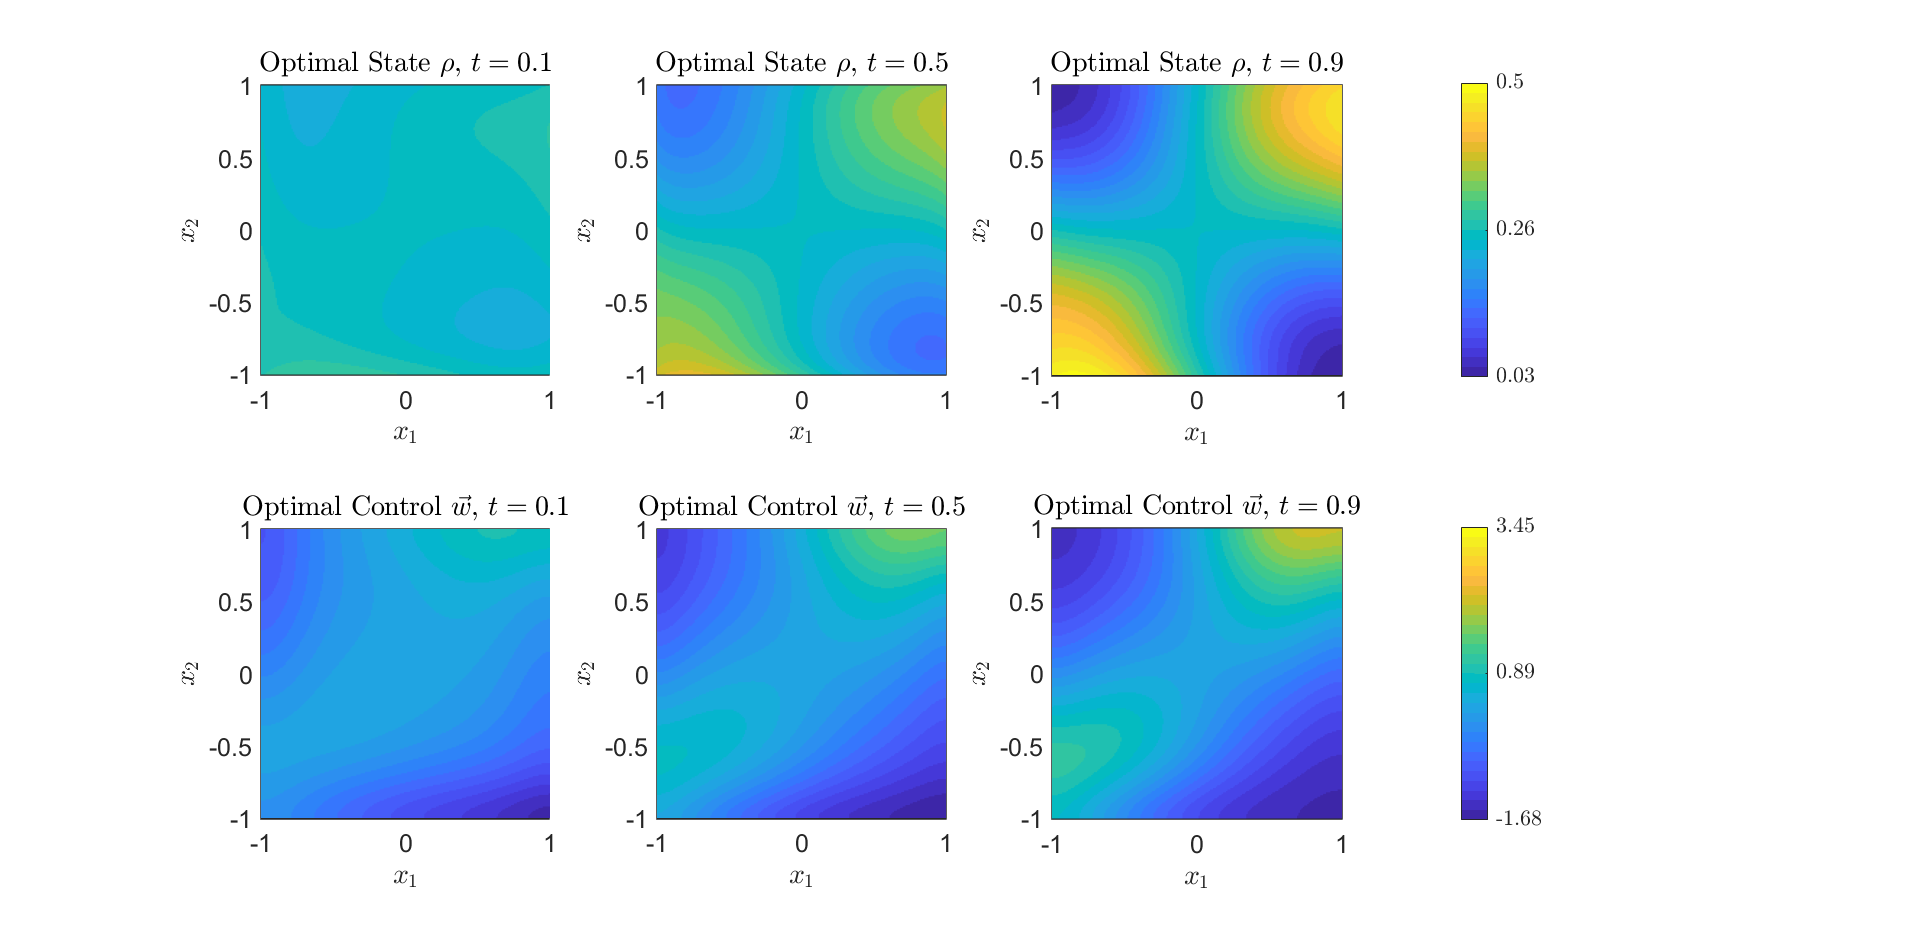
\includegraphics[scale=0.35]{SCEx1k1.png}
		\caption{Optimal $\rho$ and optimal control for $\kappa = 1$ and $\beta = 10^{-3}$.} 
		\label{F1c}
	\end{figure}
	
	\begin{figure}[h]
		\centering
		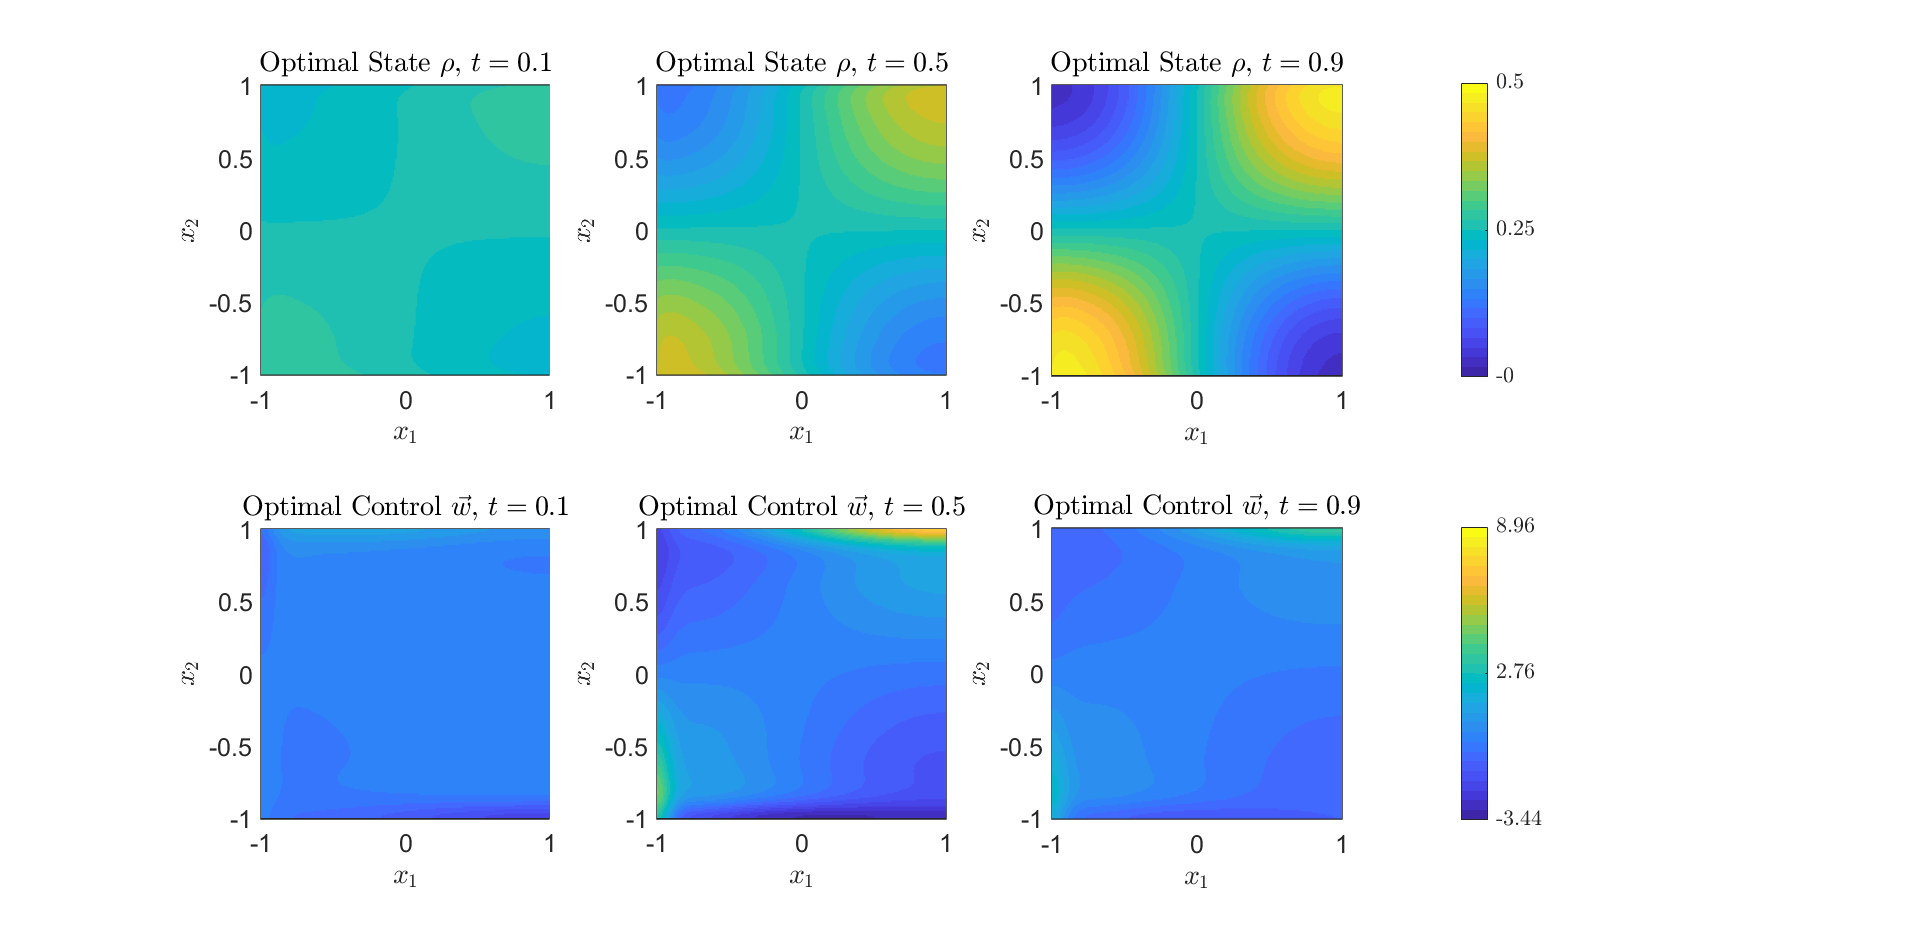
\includegraphics[scale=0.35]{SCEx1k0b5.png}
		\caption{Neumann Source Control: Optimal $\rho$ and optimal control for $\kappa = 0$ and $\beta = 10^{-5}$.} 
		\label{F1a5}
	\end{figure}
	\begin{figure}[h]
		\centering
		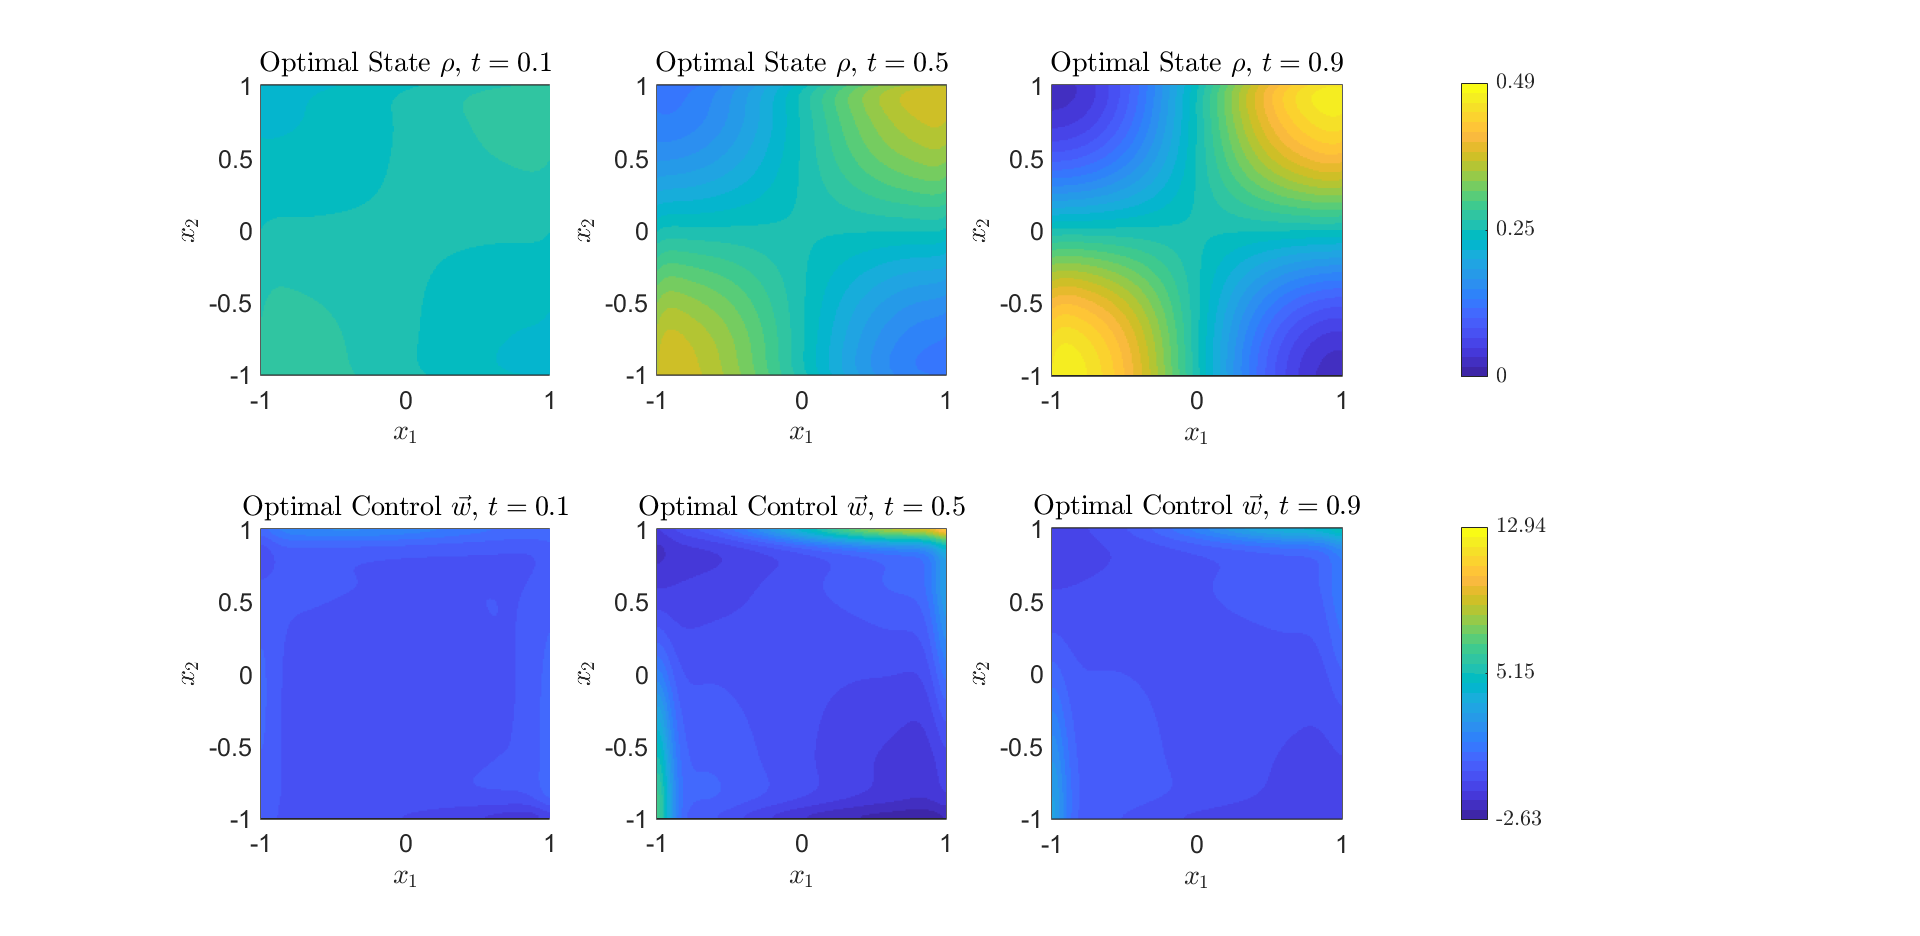
\includegraphics[scale=0.35]{SCEx1kn1b5.png}
		\caption{Neumann Source Control: Optimal $\rho$ and optimal control for $\kappa = -1$ and $\beta = 10^{-5}$.} 
		\label{F1b5}
	\end{figure}
	\begin{figure}[h]
		\centering
		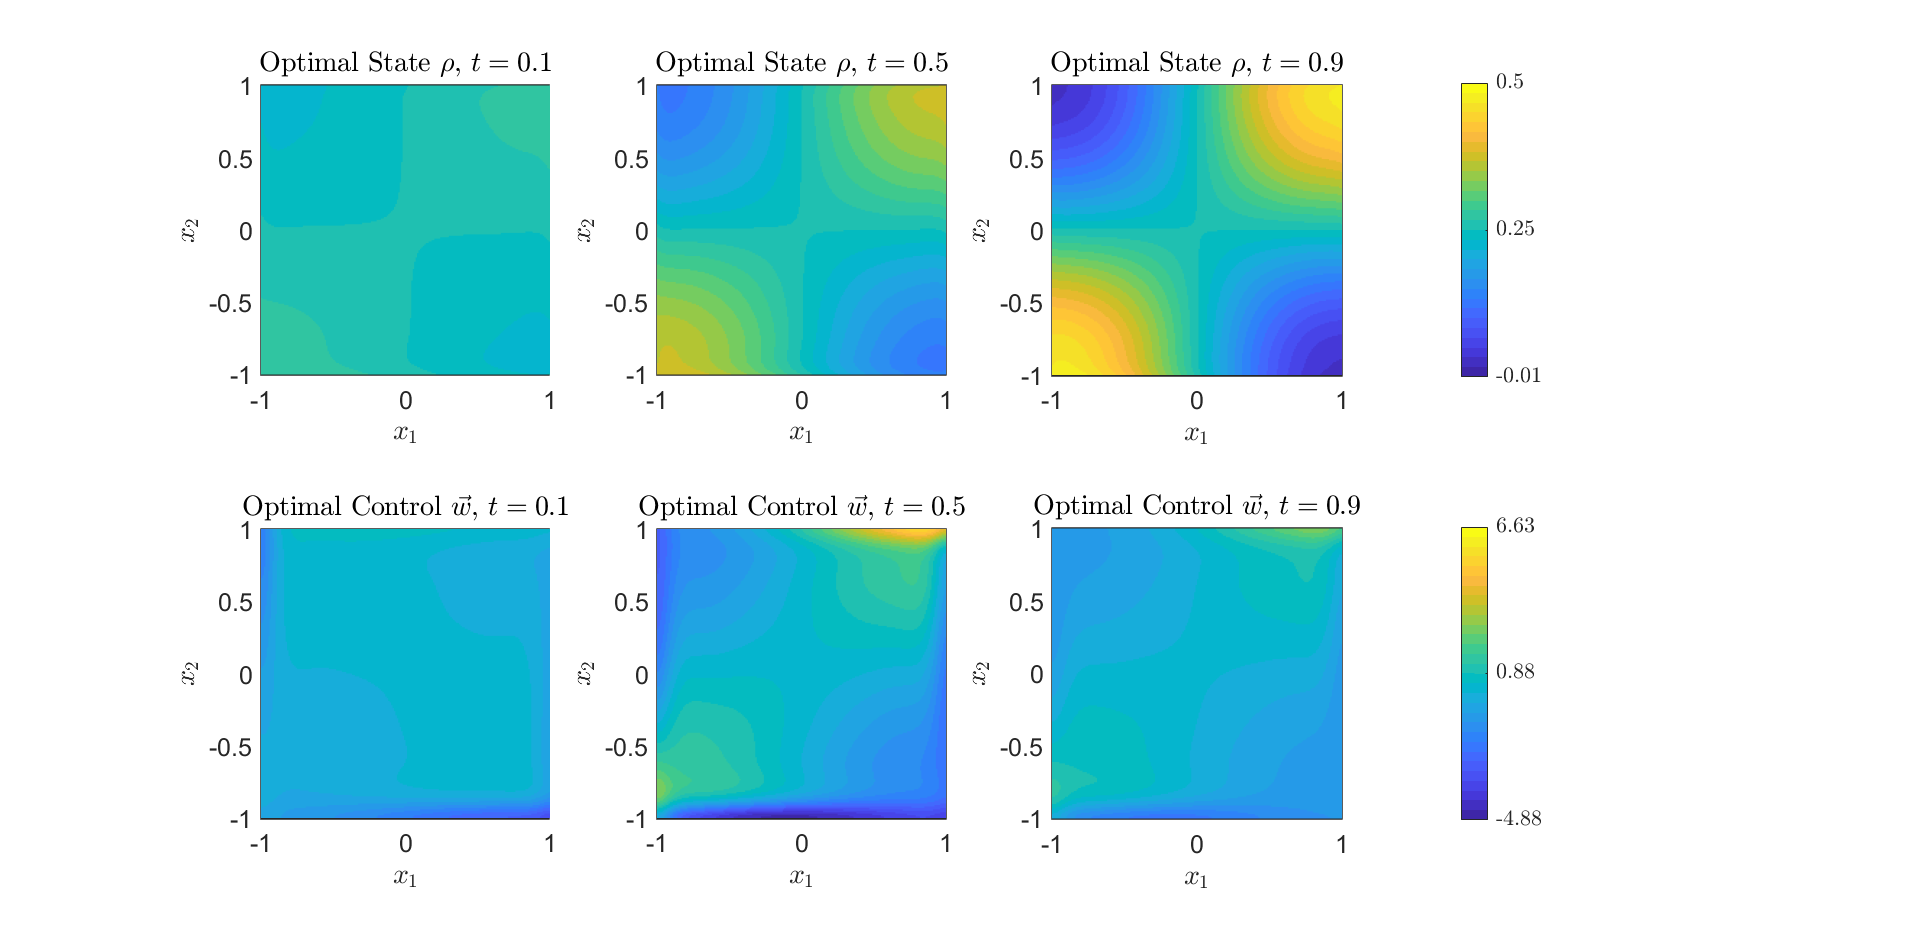
\includegraphics[scale=0.35]{SCEx1k1b5.png}
		\caption{Neumann Source Control: Optimal $\rho$ and optimal control for $\kappa = 1$ and $\beta = 10^{-5}$.} 
		\label{F1c5}
	\end{figure}
	\section*{Dirichlet Source Control}
	We choose 
	\begin{align*}
		\rho_0 &= 0.25\cos(\pi x_1/2)\cos(\pi x_2/2) + 0.25\\
		V_{ext} &=  (1-t)(-\cos(\pi x_1/2)\sin(\pi x_2/2) + 1)\\
		\hr &= 0.25\cos(\pi x_1/2)\cos(\pi x_2/2)(1 - t) - t(0.25\sin(\pi x_1)\sin(\pi x_2/2 - \pi/2) + 0.25)
	\end{align*}
	so that the problem has Dirichlet boundary conditions at $0.25$ ($\rho = 0.25$ on $\partial \Omega$).
	We choose the domain $[-1,1]^2$ with a time horizon $(0,1)$ and $N = 20$, $n = 11$.
	For $\beta = 10^{-3}$, for $\kappa = -1$ we have $\mathcal J_c = 0.0036$, for $\kappa = 0$ (compared to $\mathcal J_{uc} = 0.0219$ from $\beta = 10^3$), $\mathcal J_c = 0.0038$ and for $\kappa = 1$, $\mathcal J_c = 0.0043$. Each of these computations takes around $70$ seconds for $10$ outer iterations. The results can be seen in Figures \ref{F2a}, \ref{F2b} and \ref{F2c} and the external potential acting on $\rho$ is displayed in Figure \ref{F2V}.\\
	
	\begin{figure}[h]
		\centering
		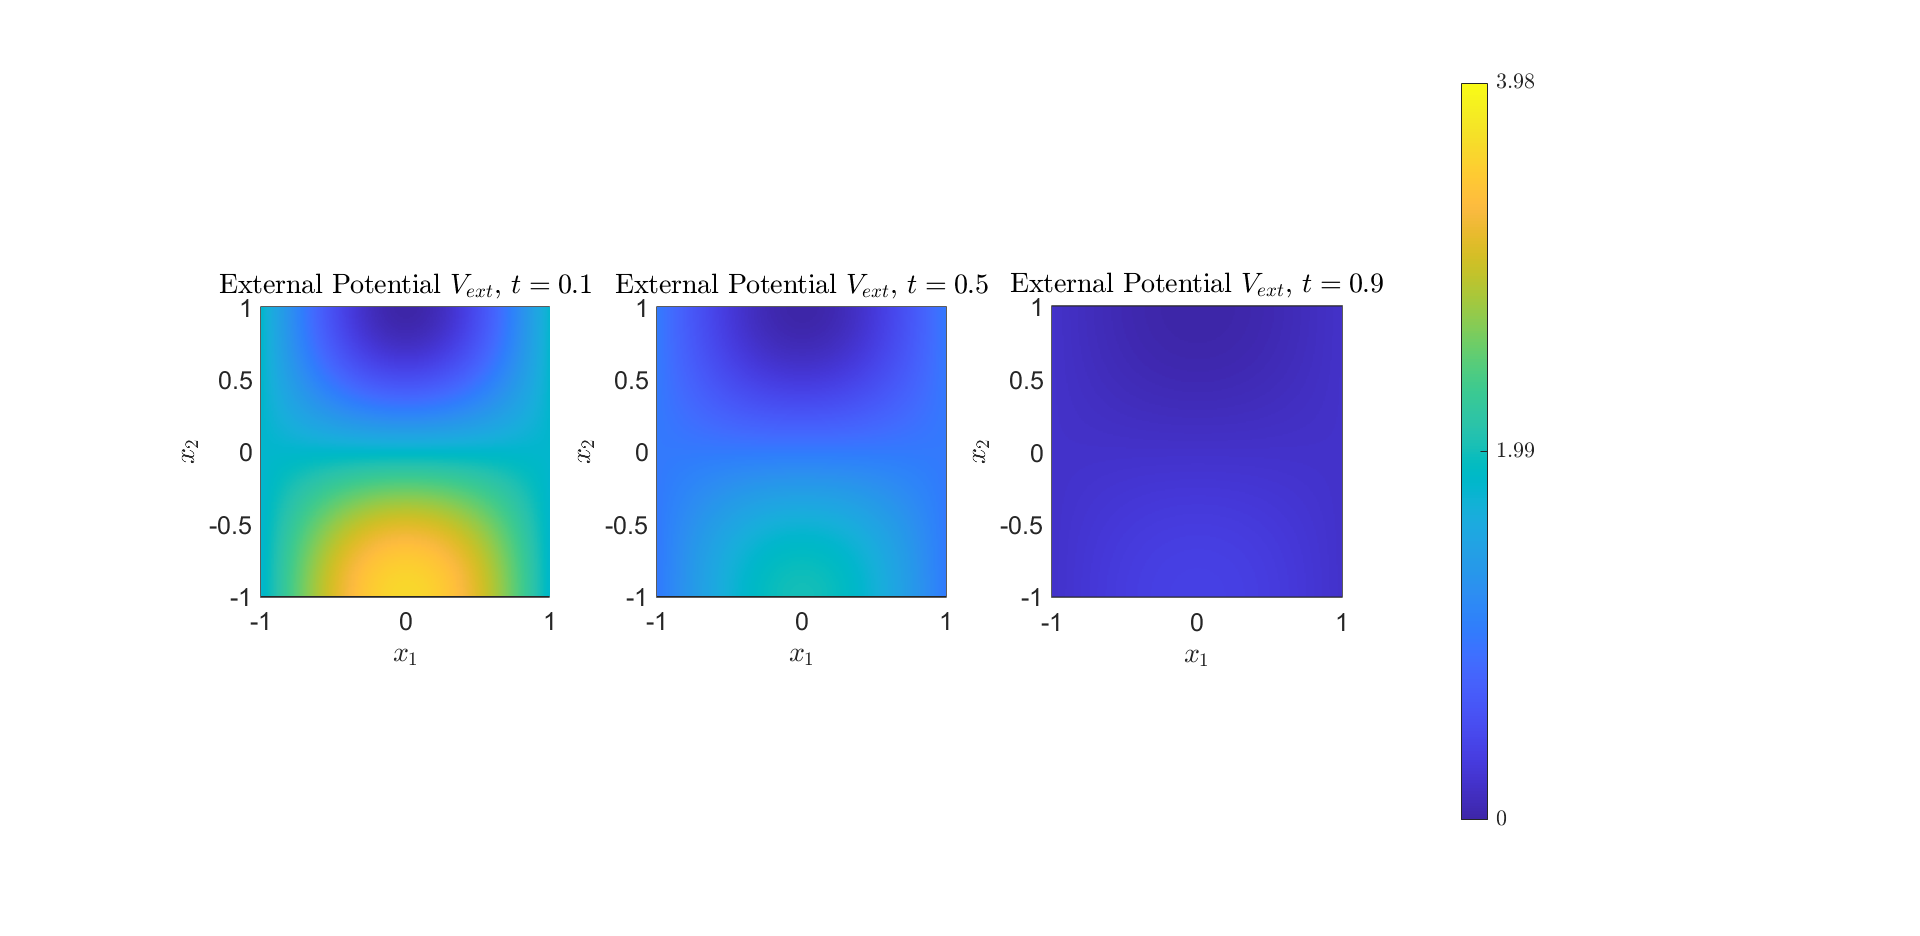
\includegraphics[scale=0.35]{SCEx2Vext.png}
		\caption{Dirichlet Source Control: External Potential $V_{ext}$ acting on $\rho$.} 
		\label{F2V}
	\end{figure}
		\begin{figure}[h]
		\centering
		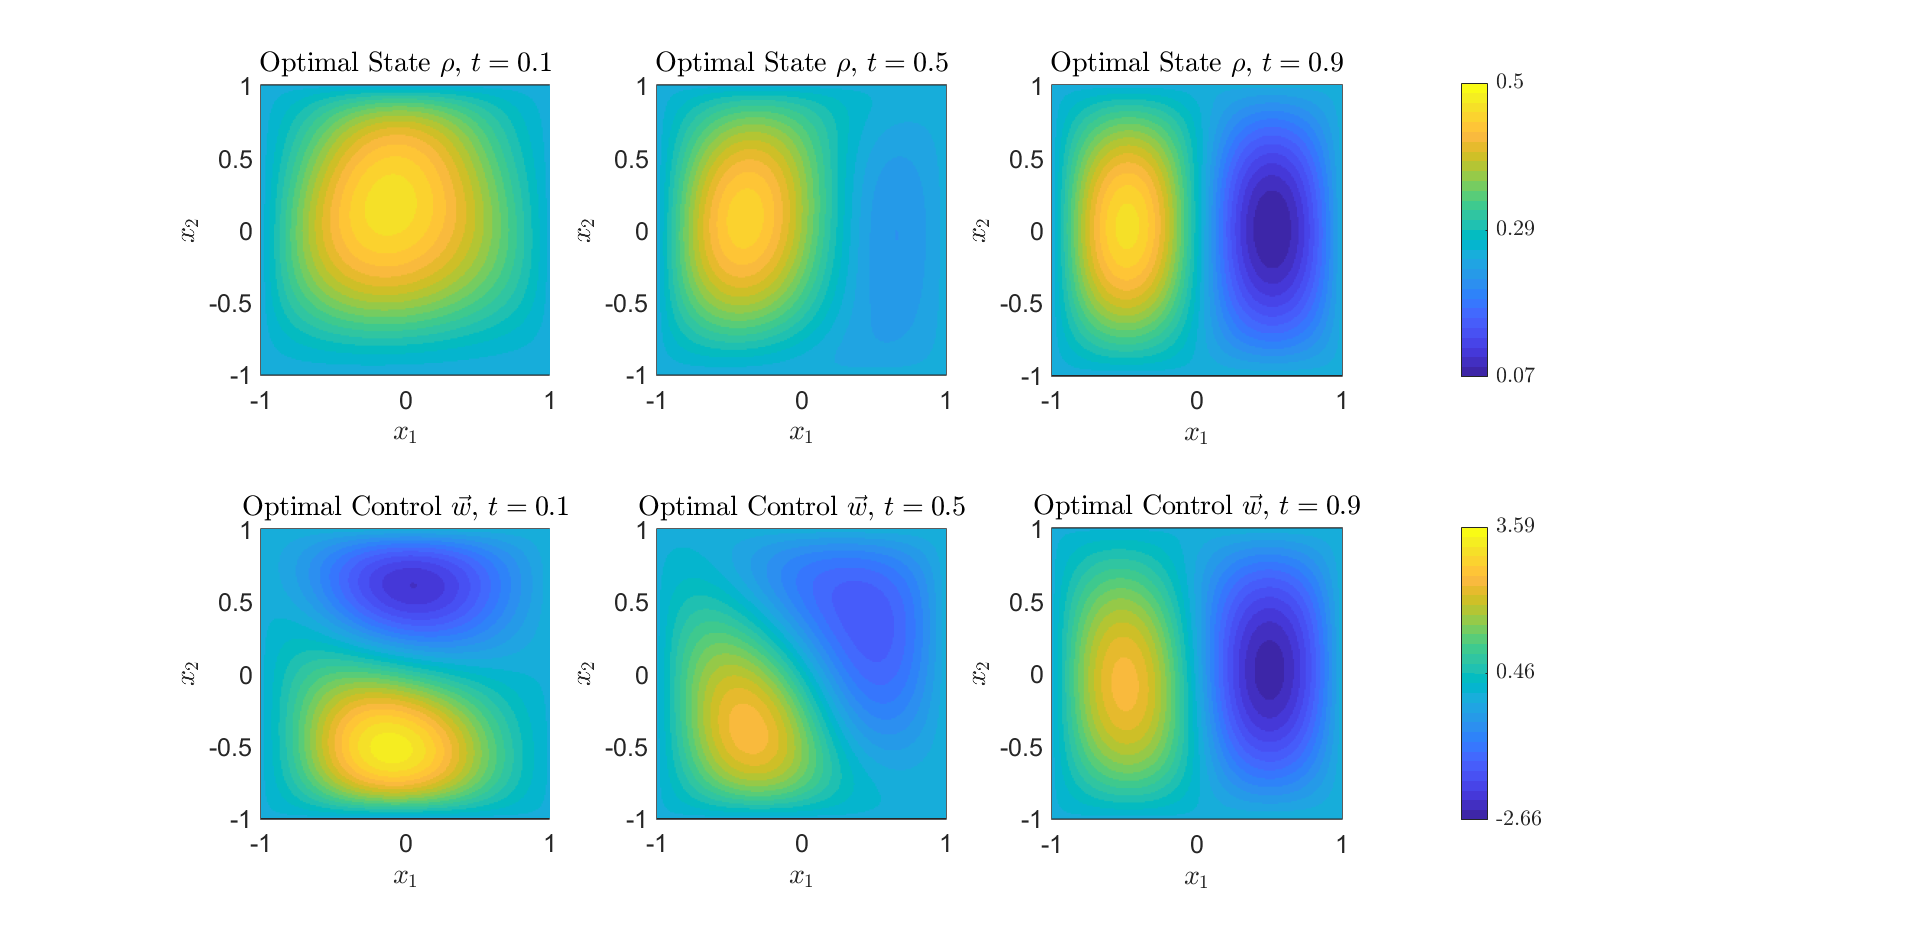
\includegraphics[scale=0.35]{SCEx2k0.png}
		\caption{Dirichlet Source Control: Optimal $\rho$ and optimal control for $\kappa = 0$ and $\beta = 10^{-3}$.} 
		\label{F2a}
	\end{figure}
	\begin{figure}[h]
		\centering
		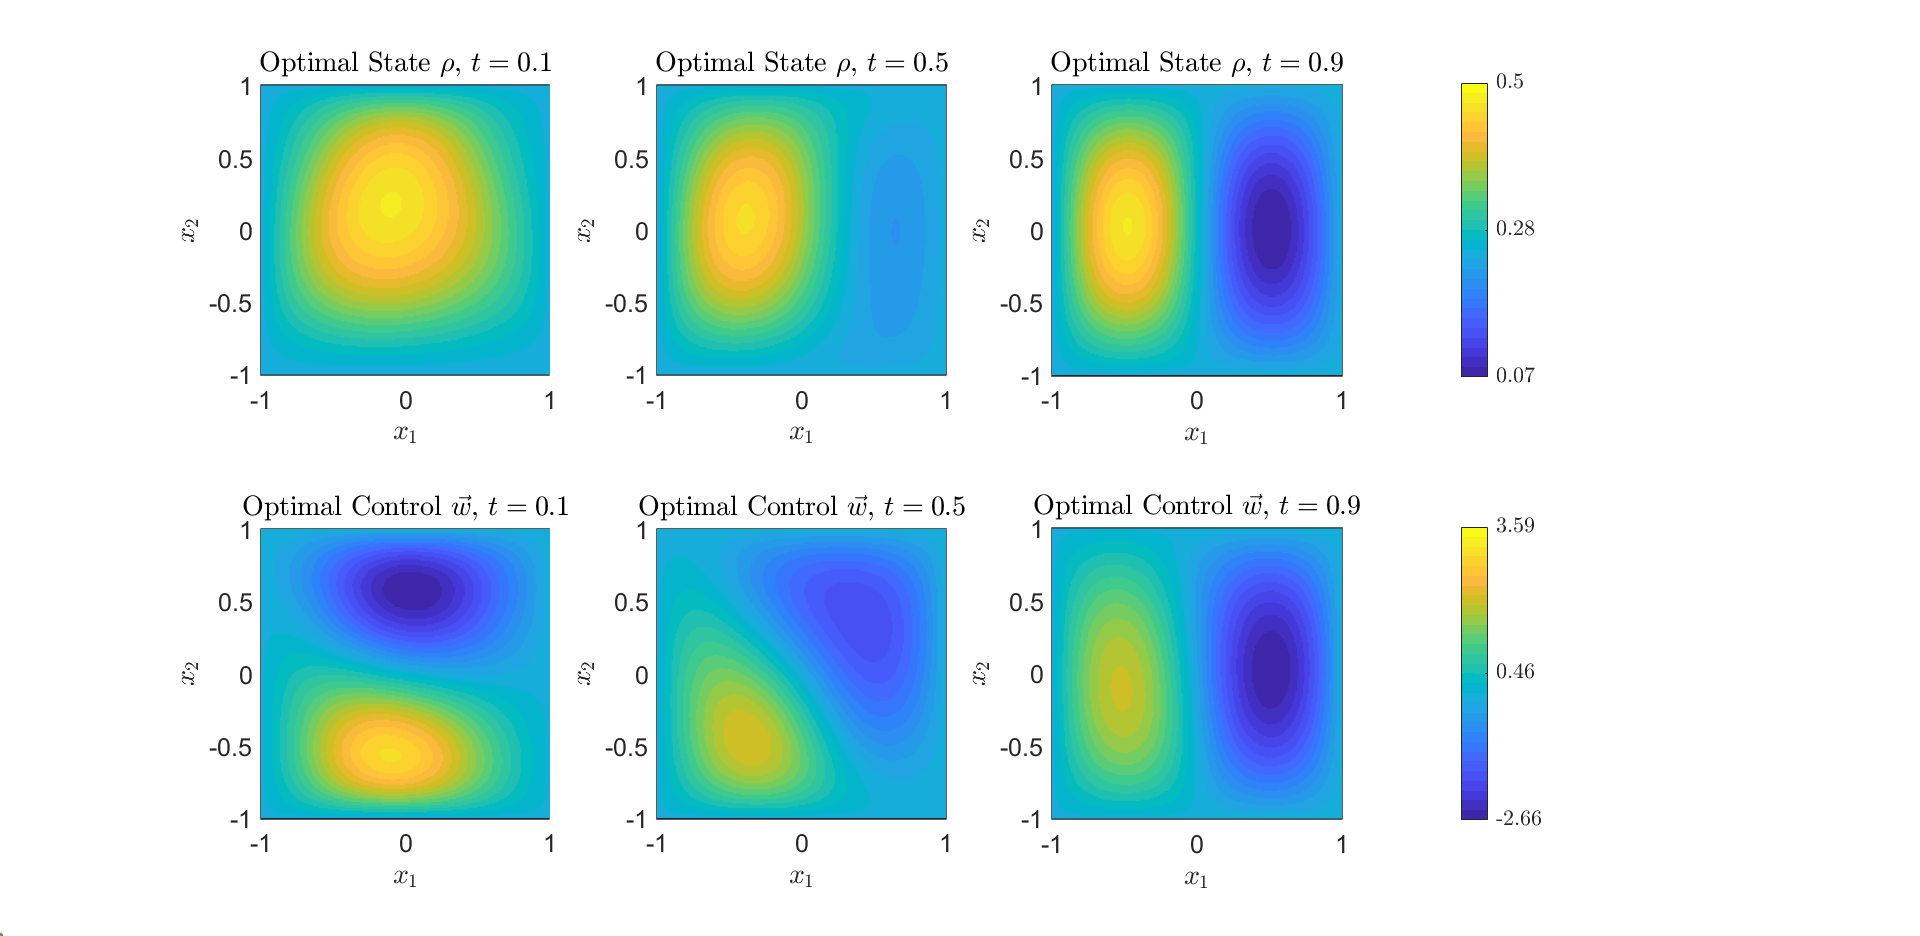
\includegraphics[scale=0.35]{SCEx2kn1.png}
		\caption{Dirichlet Source Control: Optimal $\rho$ and optimal control for $\kappa = -1$ and $\beta = 10^{-3}$.} 
		\label{F2b}
	\end{figure}
	\begin{figure}[h]
		\centering
		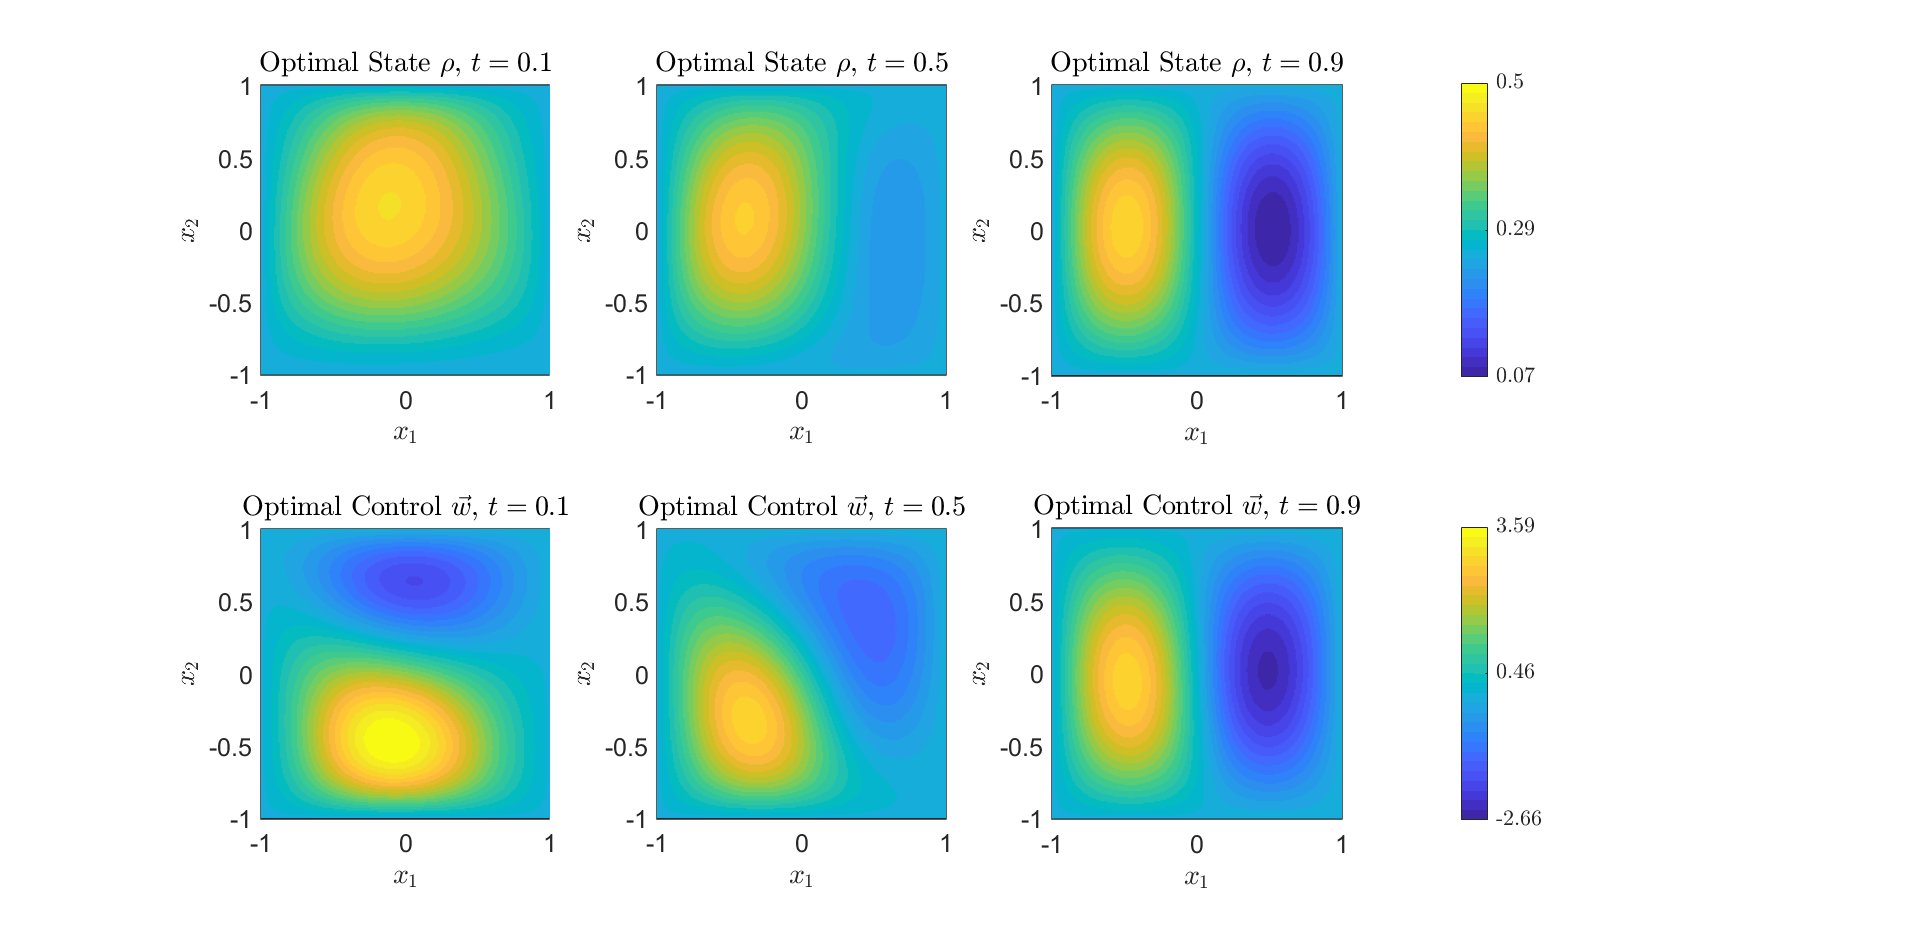
\includegraphics[scale=0.35]{SCEx2k1.png}
		\caption{Dirichlet Source Control: Optimal $\rho$ and optimal control for $\kappa = 1$ and $\beta = 10^{-3}$.} 
		\label{F2c}
	\end{figure}
	
	\section{Neumann Flow Control}
	We choose 
	\begin{align*}
		\rho_0 &= 0.25\\
		V_{ext} &= ((x_1 + 0.3)^2 - 1)((x_1-0.4)^2 - 0.5)
		((x_2 + 0.3)^2 - 1)((x_2-0.4)^2 - 0.5)\\
		\hr &= (1-t)0.25 + t(1/1.3791)\exp{(-2((x_1+0.2)^2 + (x_2+0.2)^2))}
	\end{align*}
	We choose the domain $[-1,1]^2$ with a time horizon $(0,1)$. We have $N = 20$, $n = 11$. 
	For $\beta = 10^{-3}$, $\kappa = 1$ we get $\mathcal J_c = 0.0059$ (compare to $\beta = 10^3$ with $\mathcal J_{uc} = 0.0336$), for $\kappa = 0$, $\mathcal J_c = 0.0043$, and for $\kappa = - 1$ we get $\mathcal J_c = 0.0030$, (compare to $\beta = 10^3$ with $\mathcal J_{uc} = 0.0214$). Each of the problems takes around $180$ seconds to solve. The results can be seen in Figures \ref{F3a}, \ref{F3b} and \ref{F3c} and the external potential associated with it is shown in Figure \ref{F3V}.
	\begin{figure}[h]
		\centering
		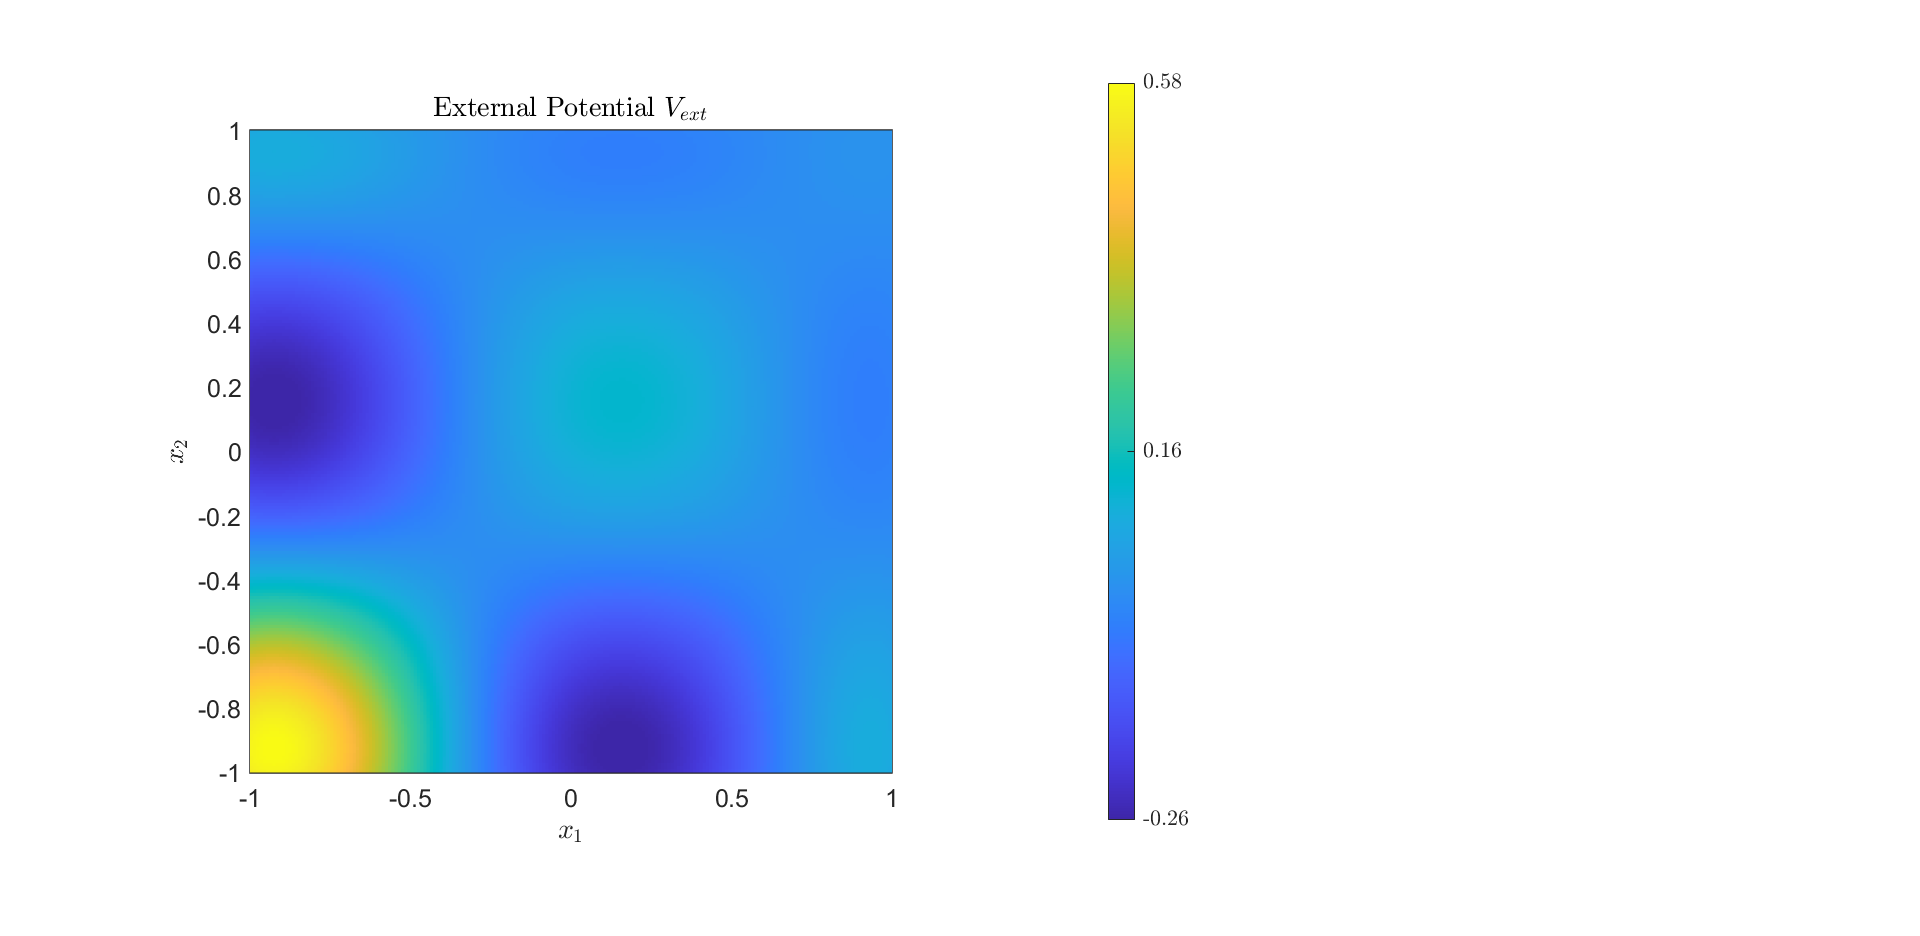
\includegraphics[scale=0.35]{FcEx1Vext.png}
		\caption{Neumann Flow Control: External Potential $V_{ext}$ acting on $\rho$.} 
		\label{F3V}
	\end{figure}
	\begin{figure}[h]
		\centering
		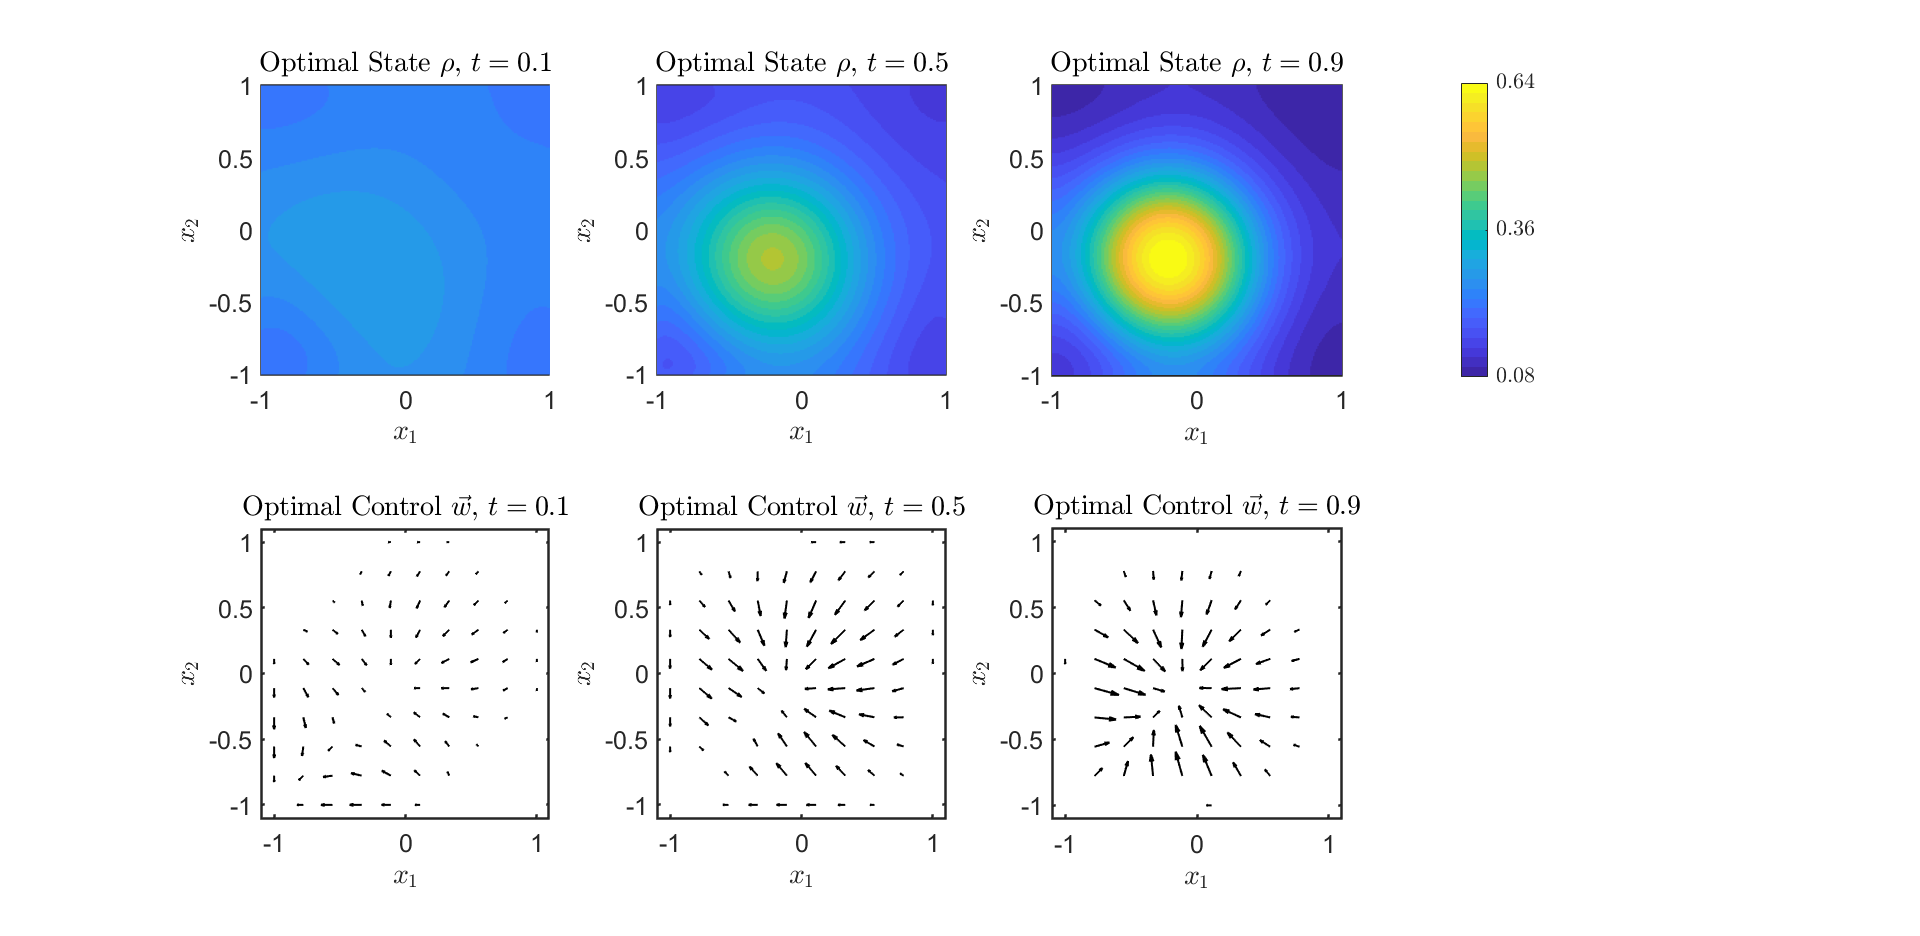
\includegraphics[scale=0.35]{FcEx1k0.png}
		\caption{Neumann Flow Control: Optimal $\rho$ and optimal control for $\kappa = 0$ and $\beta = 10^{-3}$.} 
		\label{F3a}
	\end{figure}
	\begin{figure}[h]
		\centering
		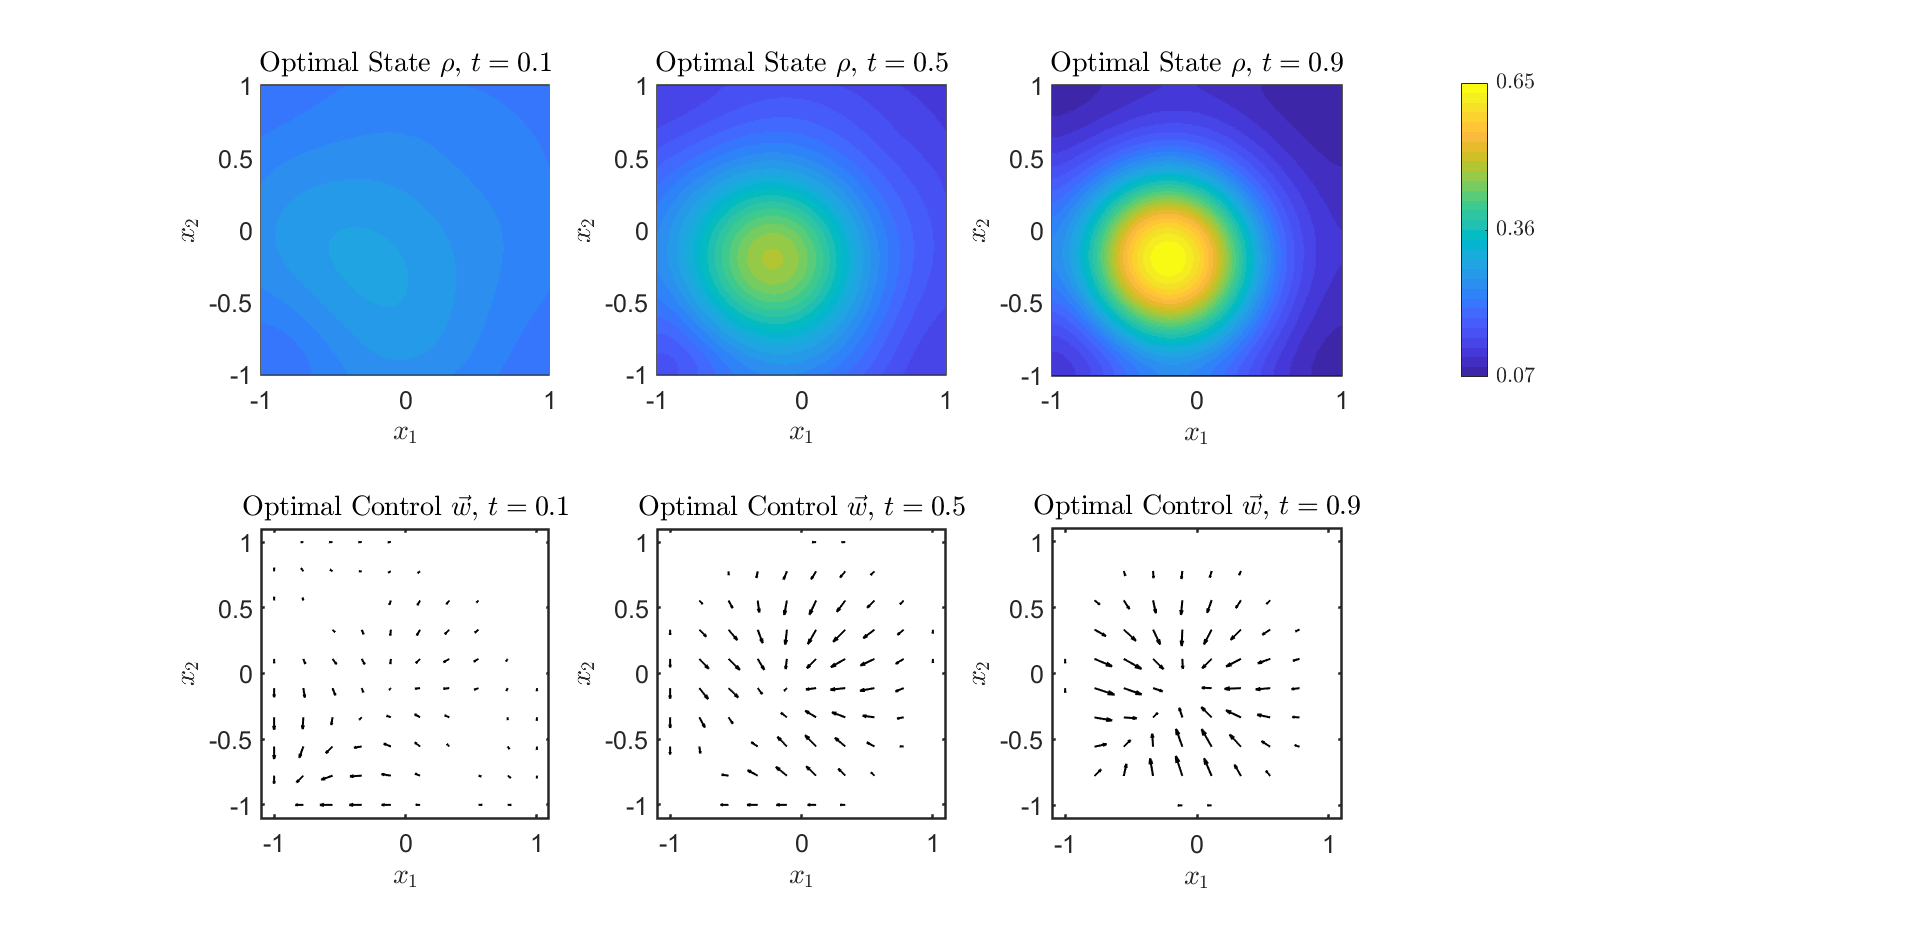
\includegraphics[scale=0.35]{FcEx1kn1.png}
		\caption{Neumann Flow Control: Optimal $\rho$ and optimal control for $\kappa = -1$ and $\beta = 10^{-3}$.} 
		\label{F3b}
	\end{figure}
	\begin{figure}[h]
		\centering
		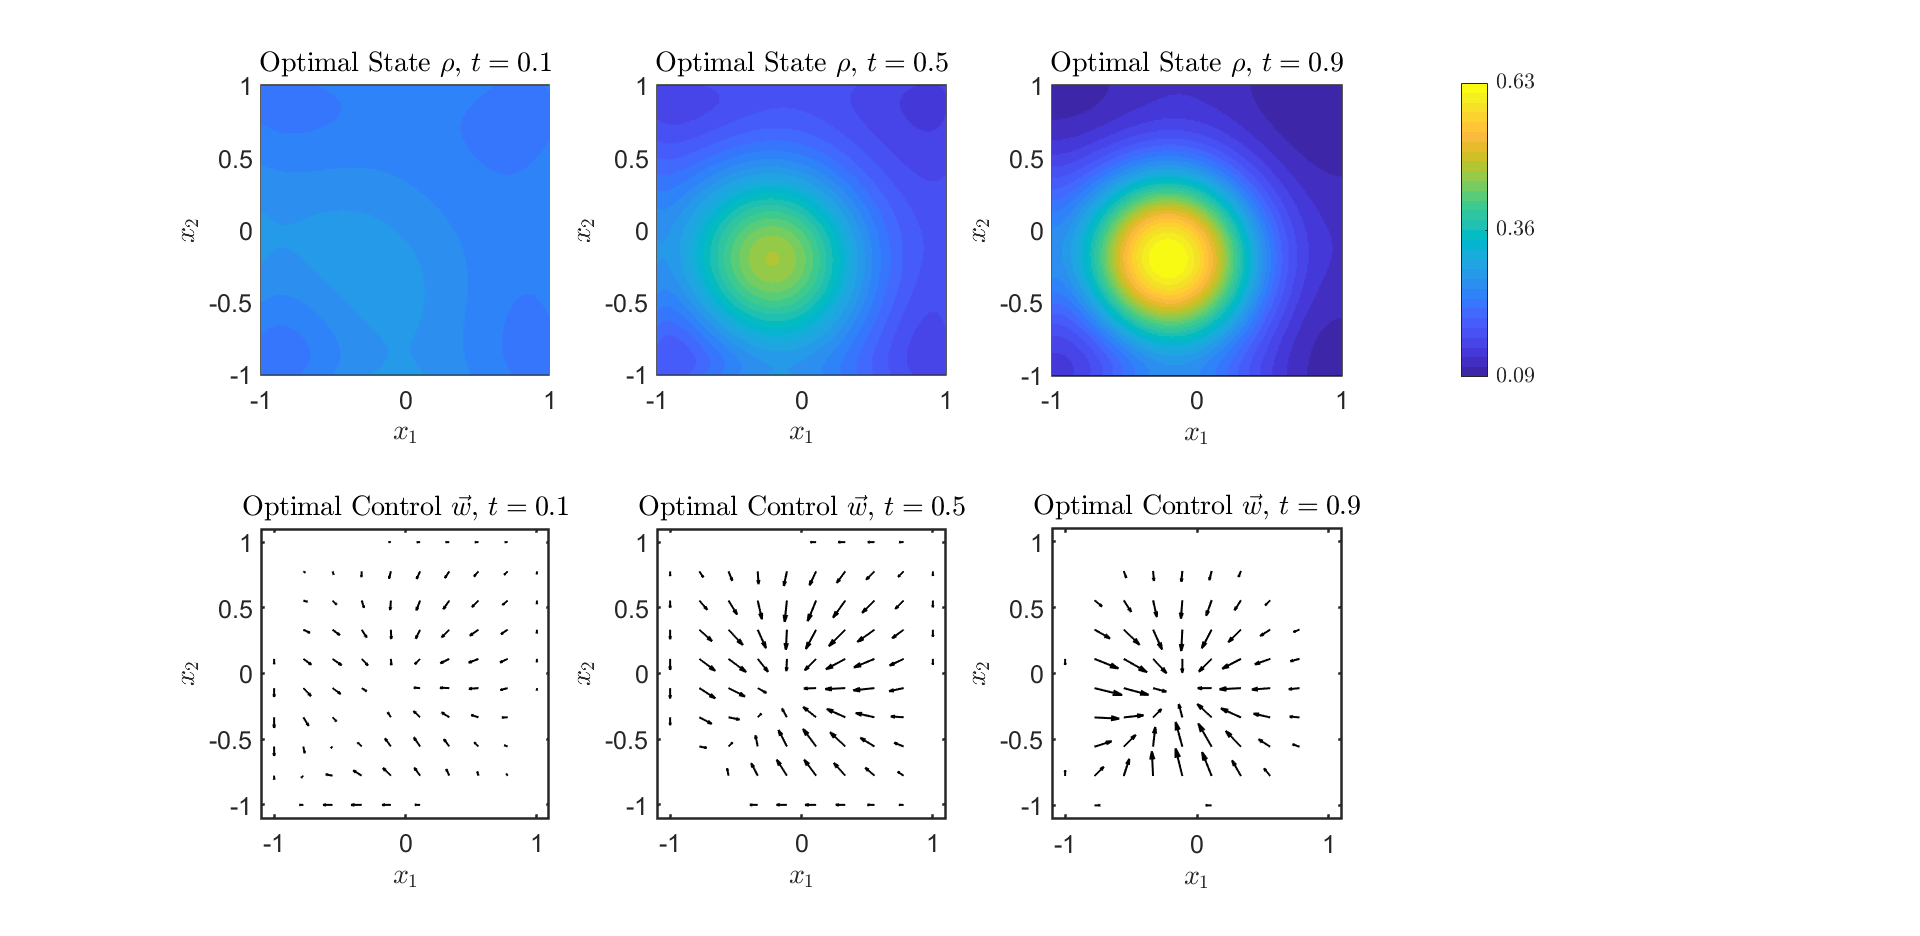
\includegraphics[scale=0.35]{FcEx1k1.png}
		\caption{Neumann Flow Control: Optimal $\rho$ and optimal control for $\kappa = 1$ and $\beta = 10^{-3}$.} 
		\label{F3c}
	\end{figure}
	
	
	\section{Dirichlet Flow Control without $V_{ext}$}
	We choose 
	\begin{align*}
		\rho_0 &= (0.25\pi)^2\cos(\pi x_1/2)\cos(\pi x_2/2) + (0.25\pi)^2\\
		\hr &= (1 - t)((0.25\pi)^2\cos(\pi x_1/2)\cos(\pi x_2/2) + (0.25\pi)^2) + t((0.25\pi)^2\cos(\pi x_1/2)\cos(3\pi x_2/2) + (0.25\pi)^2)
	\end{align*}
	We choose the domain $[-1,1]^2$ with a time horizon $(0,1)$. We have $N = 20$, $n = 11$. 
	For $\beta = 10^{-3}$, $\kappa = 1$ we get $\mathcal J_c = 0.0121$, for $\kappa = 0$, $\mathcal J_c = 0.0095$, and for $\kappa = - 1$ we get $\mathcal J_c = 0.0104$, (compare to $\beta = 10^3$ with $\mathcal J_{uc} = 0.5272$). Each of the problems takes around $50$ seconds to solve. The results can be seen in Figures \ref{F4a}, \ref{F4b} and \ref{F4c}.


%		\begin{figure}[h]
%		\centering
%		\includegraphics[scale=0.35]{FcEx2Vext.png}
%		\caption{Dirichlet Flow Control: External Potential $V_{ext}$ acting on $\rho$.} 
%		\label{F4V}
%	\end{figure}
	\begin{figure}[h]
		\centering
		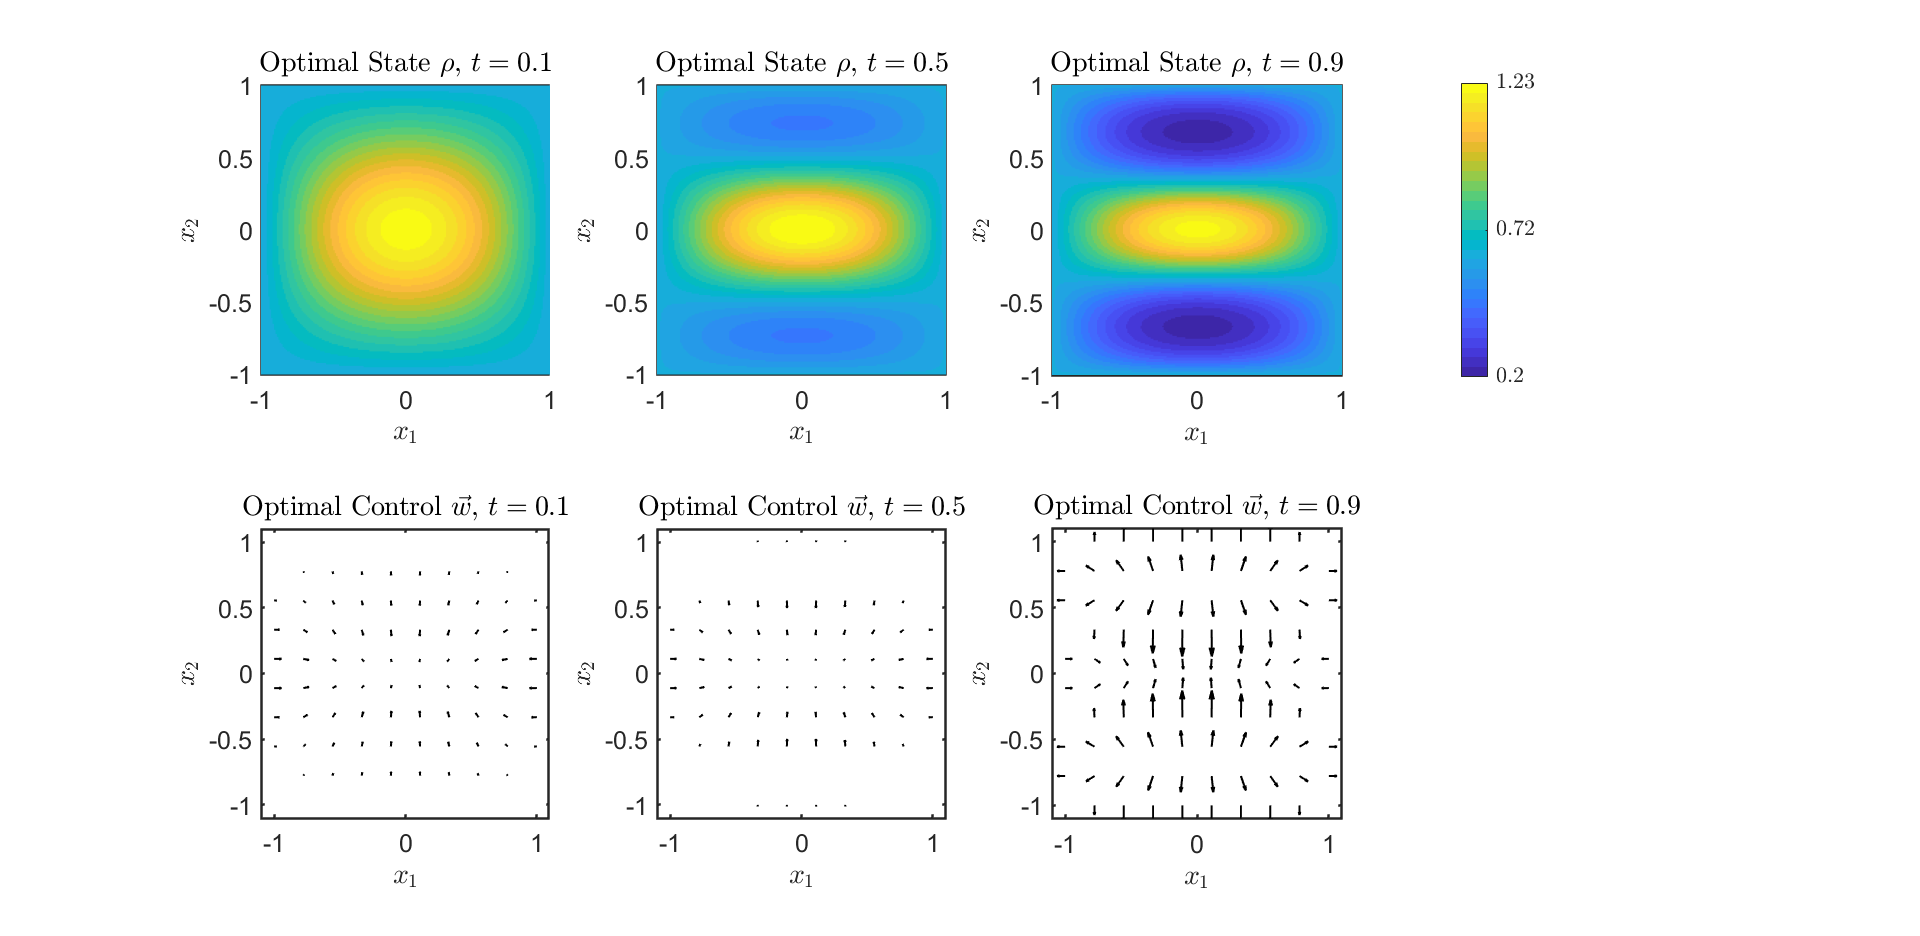
\includegraphics[scale=0.35]{FcEx2k0.png}
		\caption{Dirichlet Flow Control: Optimal $\rho$ and optimal control for $\kappa = 0$ and $\beta = 10^{-3}$.} 
		\label{F4a}
	\end{figure}
	\begin{figure}[h]
		\centering
		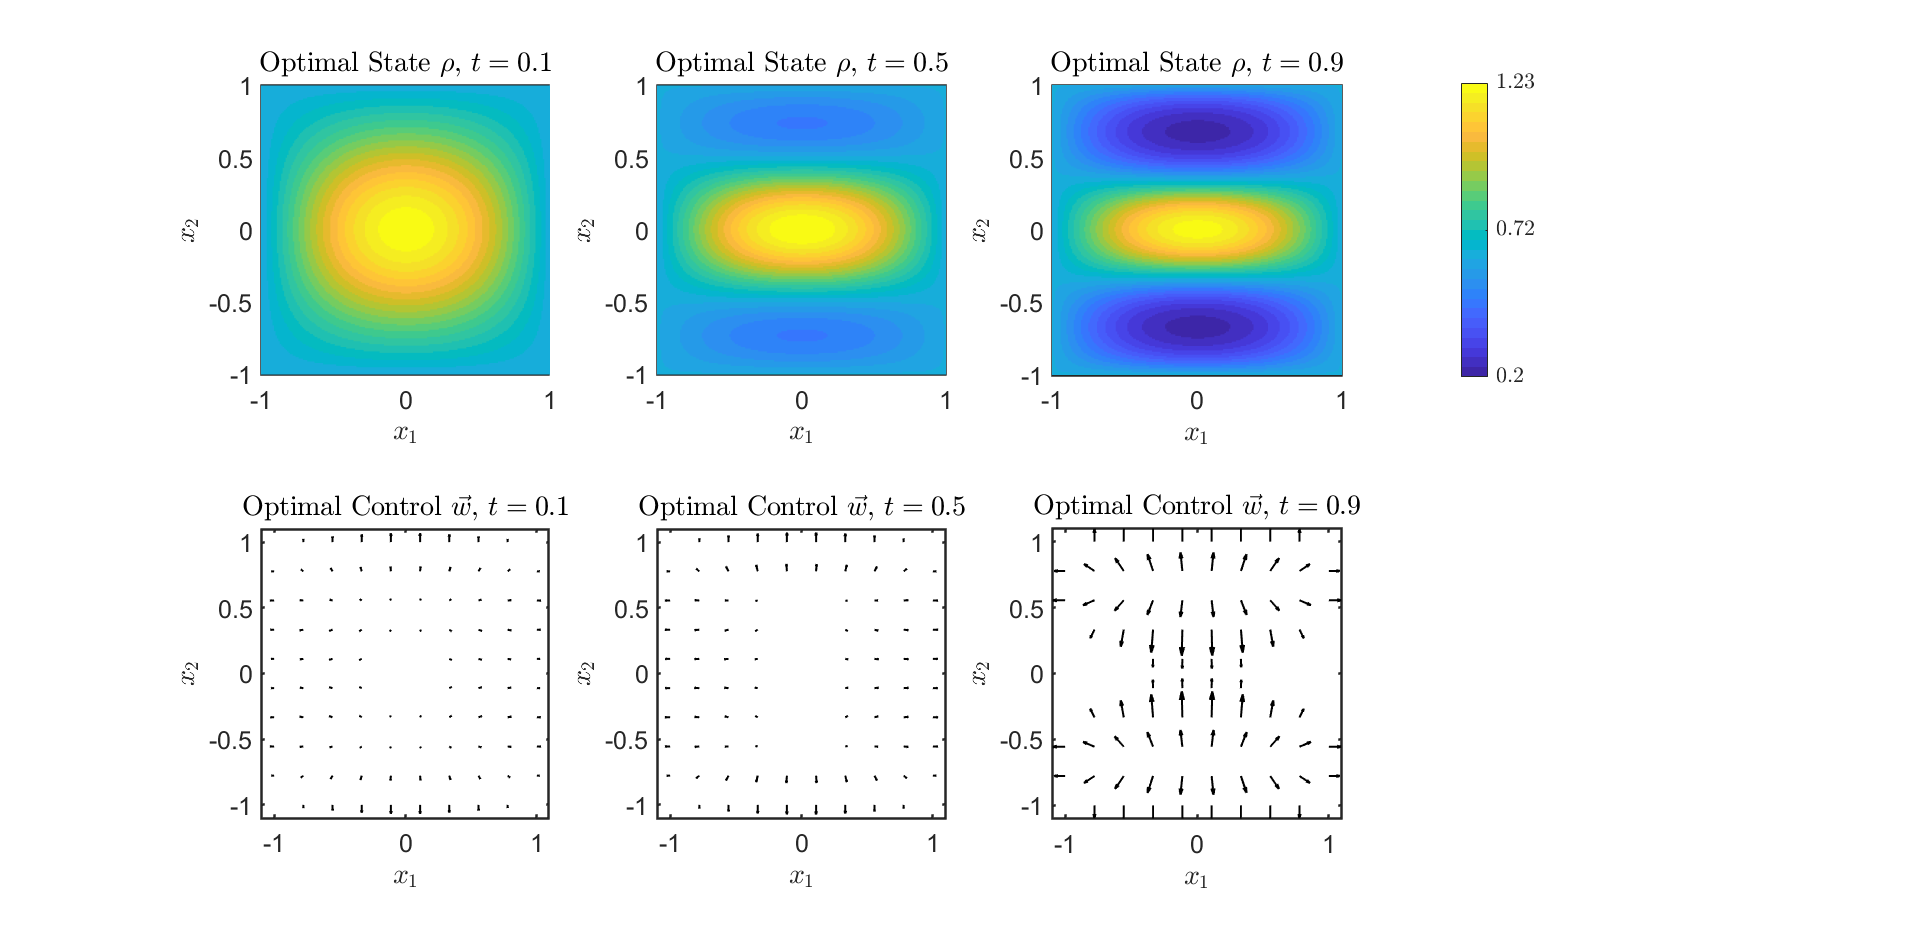
\includegraphics[scale=0.35]{FcEx2kn1.png}
		\caption{Dirichlet Flow Control: Optimal $\rho$ and optimal control for $\kappa = -1$ and $\beta = 10^{-3}$.} 
		\label{F4b}
	\end{figure}
	\begin{figure}[h]
		\centering
		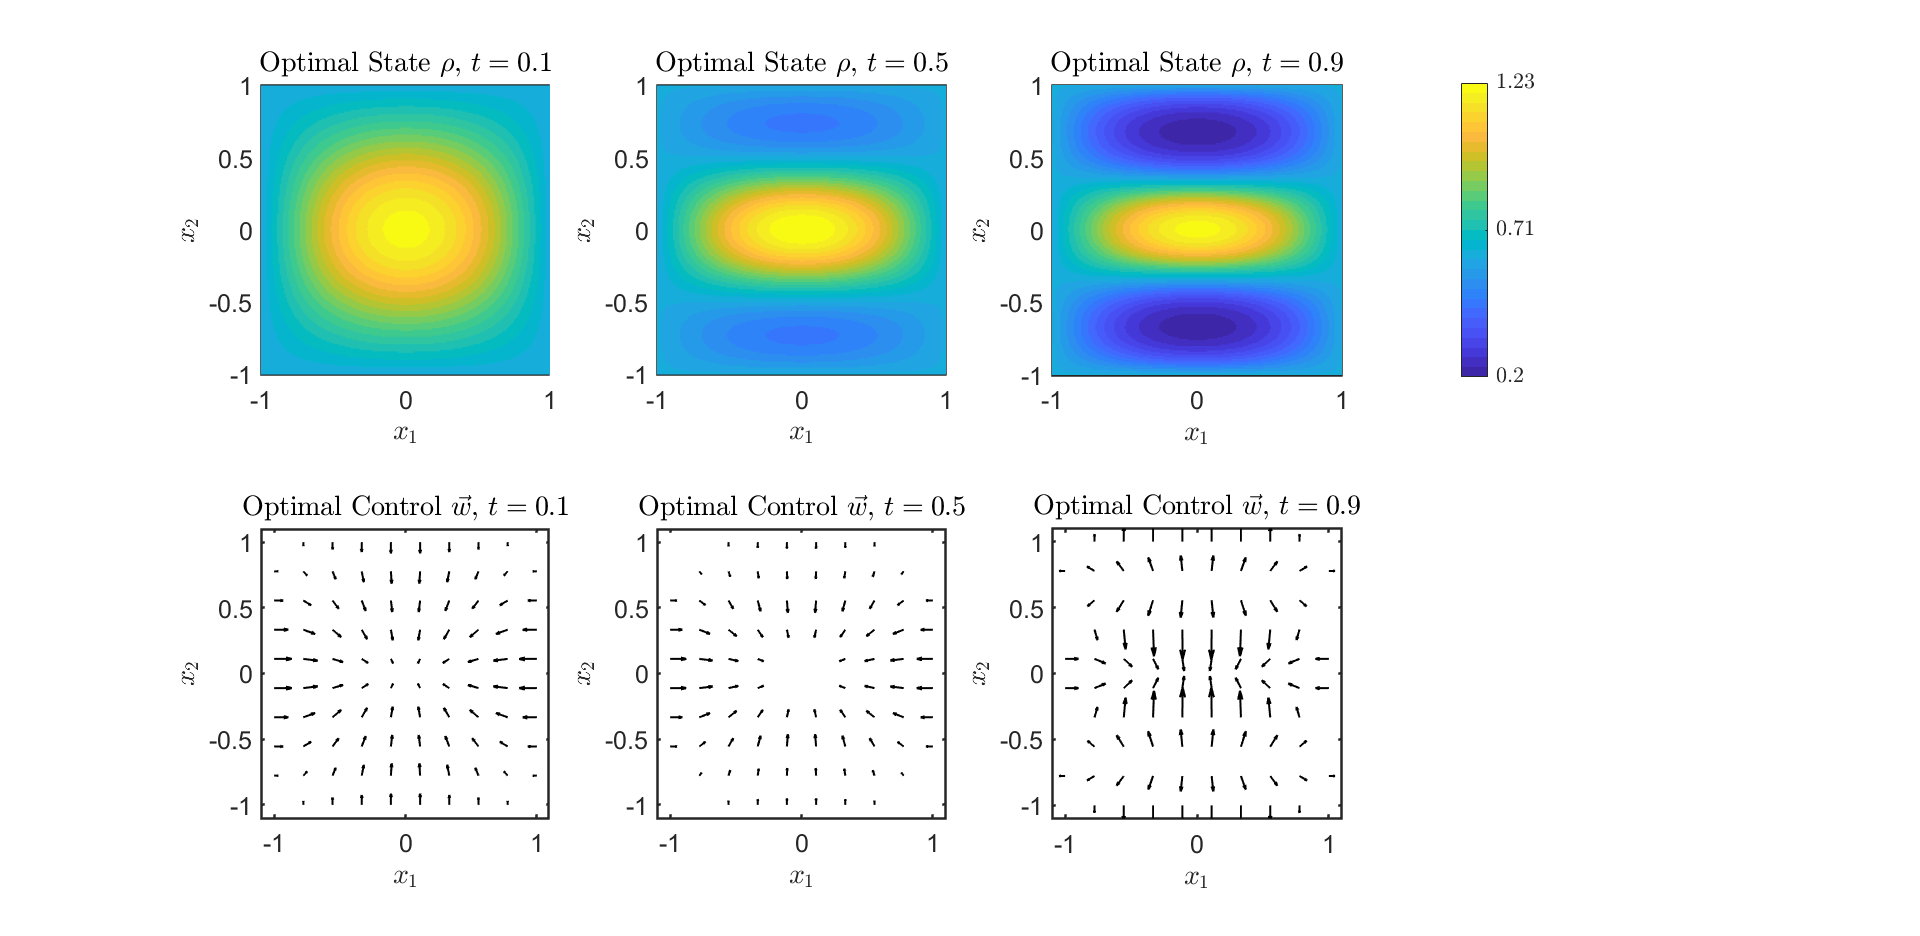
\includegraphics[scale=0.35]{FcEx2k1.png}
		\caption{Dirichlet Flow Control: Optimal $\rho$ and optimal control for $\kappa = 1$ and $\beta = 10^{-3}$.} 
		\label{F4c}
	\end{figure}
	
		\section{Dirichlet Flow Control with $V_{ext}$}
	We add the following external potential to the above problem, see Figure \ref{F5V} 
	\begin{align*}
		V_{ext} = 10\sin(\pi x_2/3 - \pi/2)\sin(\pi x_1/2)
	\end{align*}
	For $\beta = 10^{-3}$, $\kappa = 1$ we get $\mathcal J_c = 0.0130$, for $\kappa = 0$, $\mathcal J_c = 0.0106$, and for $\kappa = - 1$ we get $\mathcal J_c = 0.0113$. (Compare these to $\beta = 10^3$ with $\mathcal J_{uc} = 0.0898$) Each of the problems takes around $50$ seconds to solve. The results can be seen in Figures \ref{F5a}, \ref{F5b} and \ref{F5c}.
	
	
	\begin{figure}[h]
		\centering
		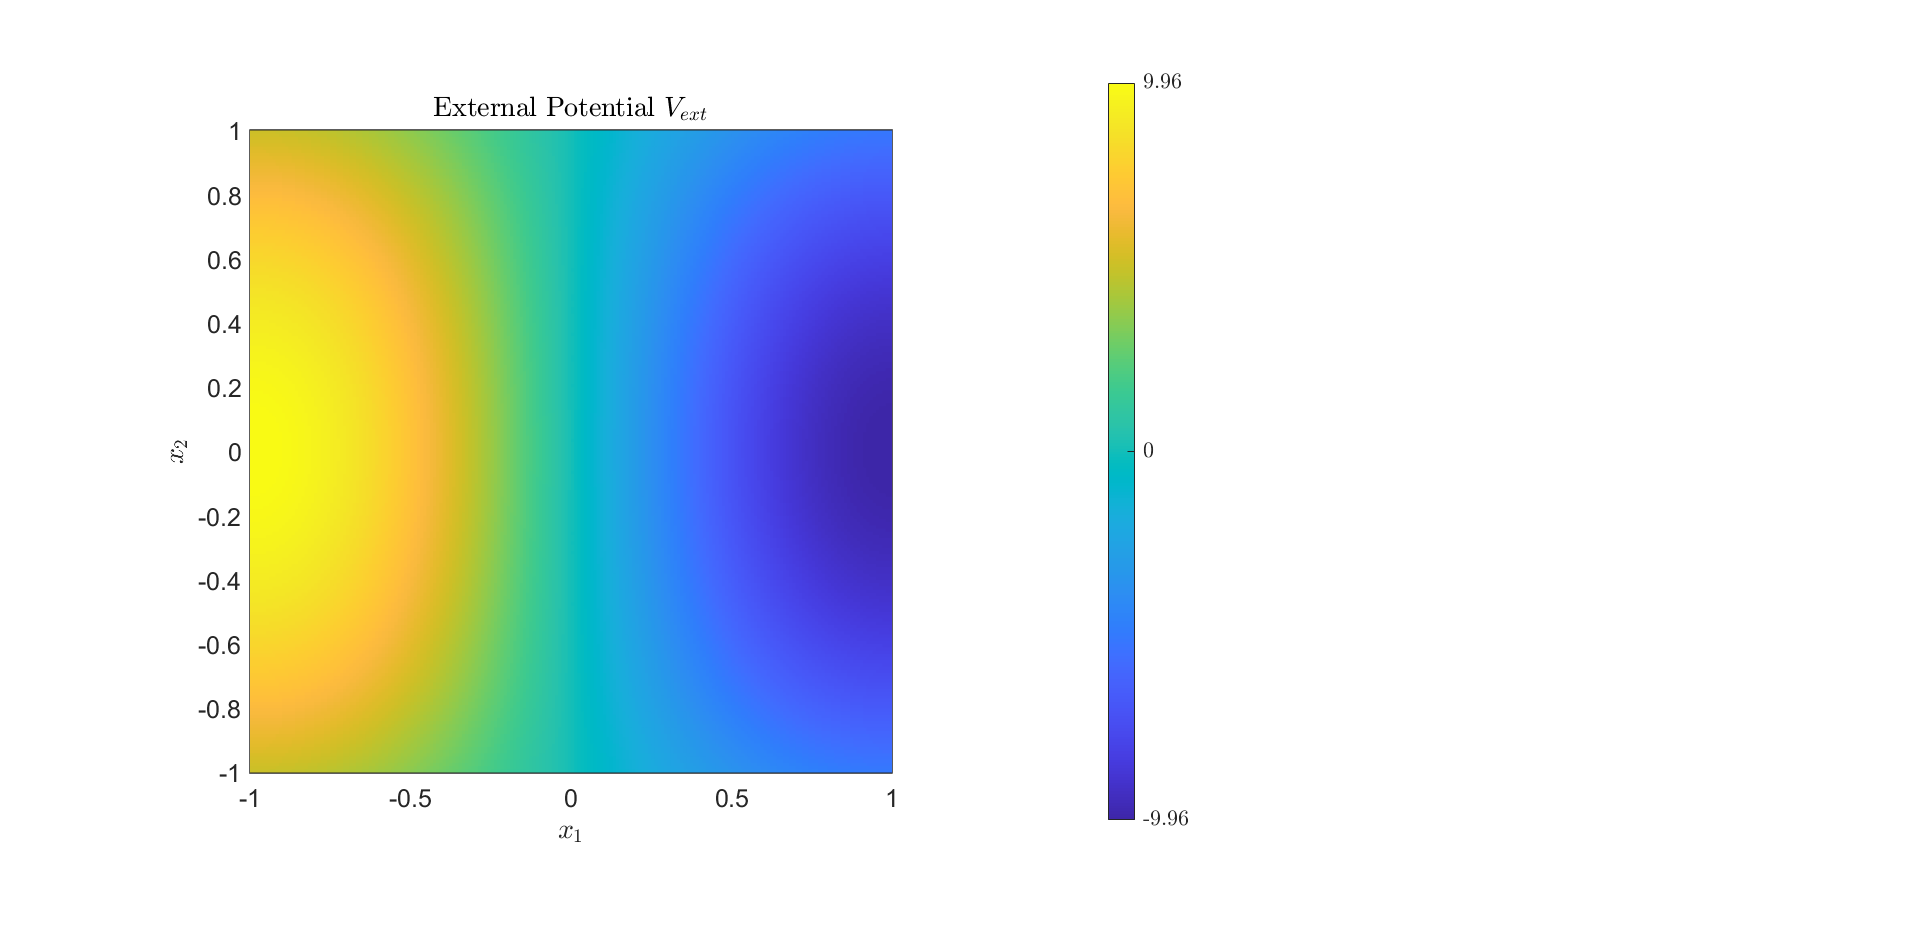
\includegraphics[scale=0.35]{FcEx2Vextb.png}
		\caption{Dirichlet Flow Control 2: External Potential $V_{ext}$ acting on $\rho$.} 
		\label{F5V}
	\end{figure}
	\begin{figure}[h]
		\centering
		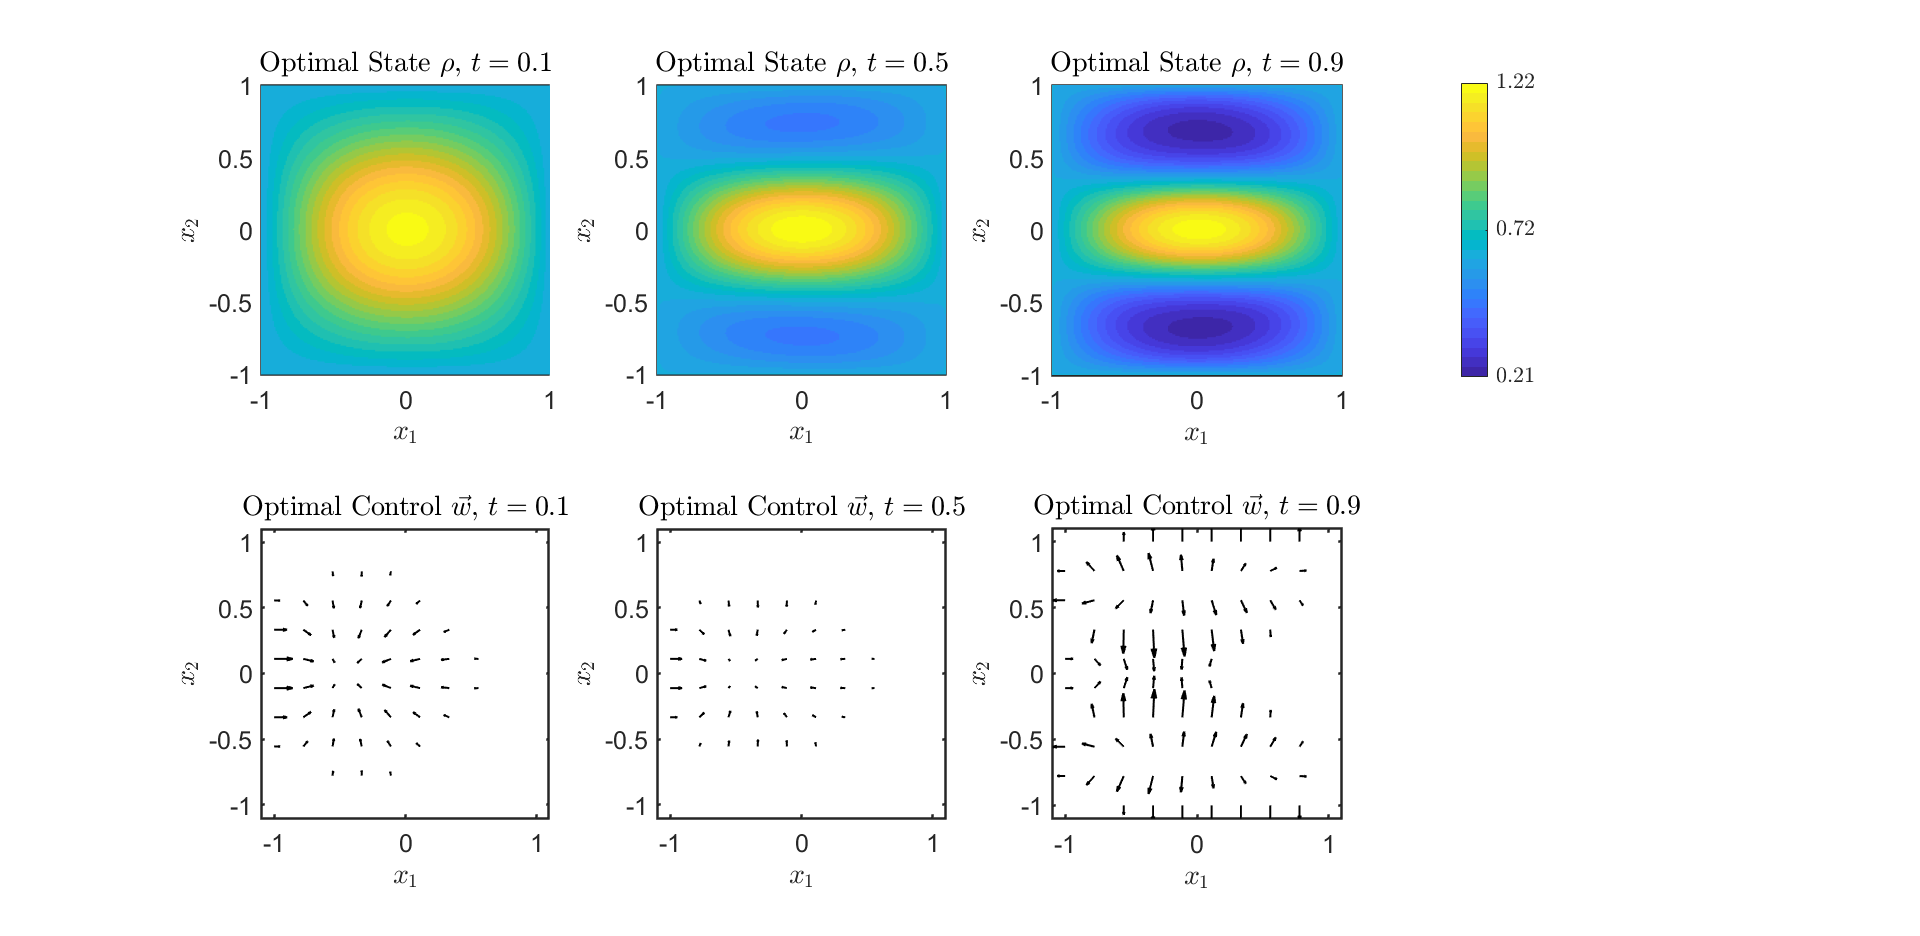
\includegraphics[scale=0.35]{FcEx2k0b.png}
		\caption{Dirichlet Flow Control 2: Optimal $\rho$ and optimal control for $\kappa = 0$ and $\beta = 10^{-3}$.} 
		\label{F5a}
	\end{figure}
	\begin{figure}[h]
		\centering
		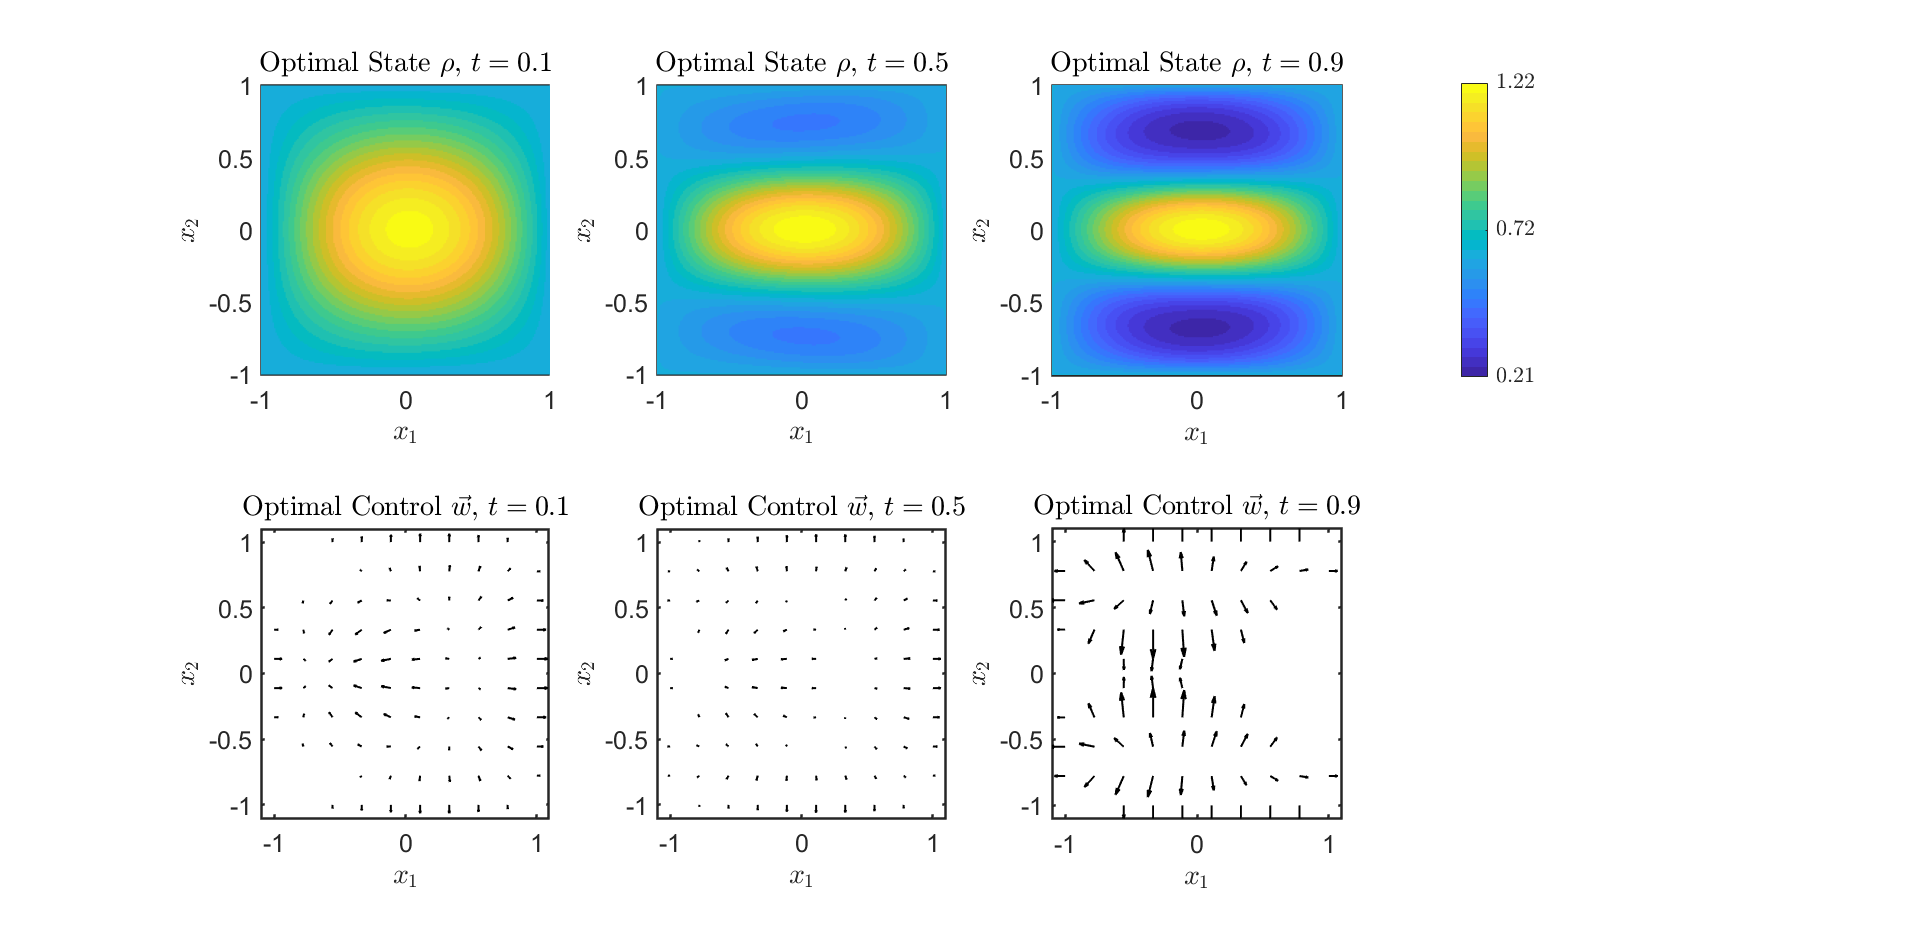
\includegraphics[scale=0.35]{FcEx2kn1b.png}
		\caption{Dirichlet Flow Control 2: Optimal $\rho$ and optimal control for $\kappa = -1$ and $\beta = 10^{-3}$.} 
		\label{F5b}
	\end{figure}
	\begin{figure}[h]
		\centering
		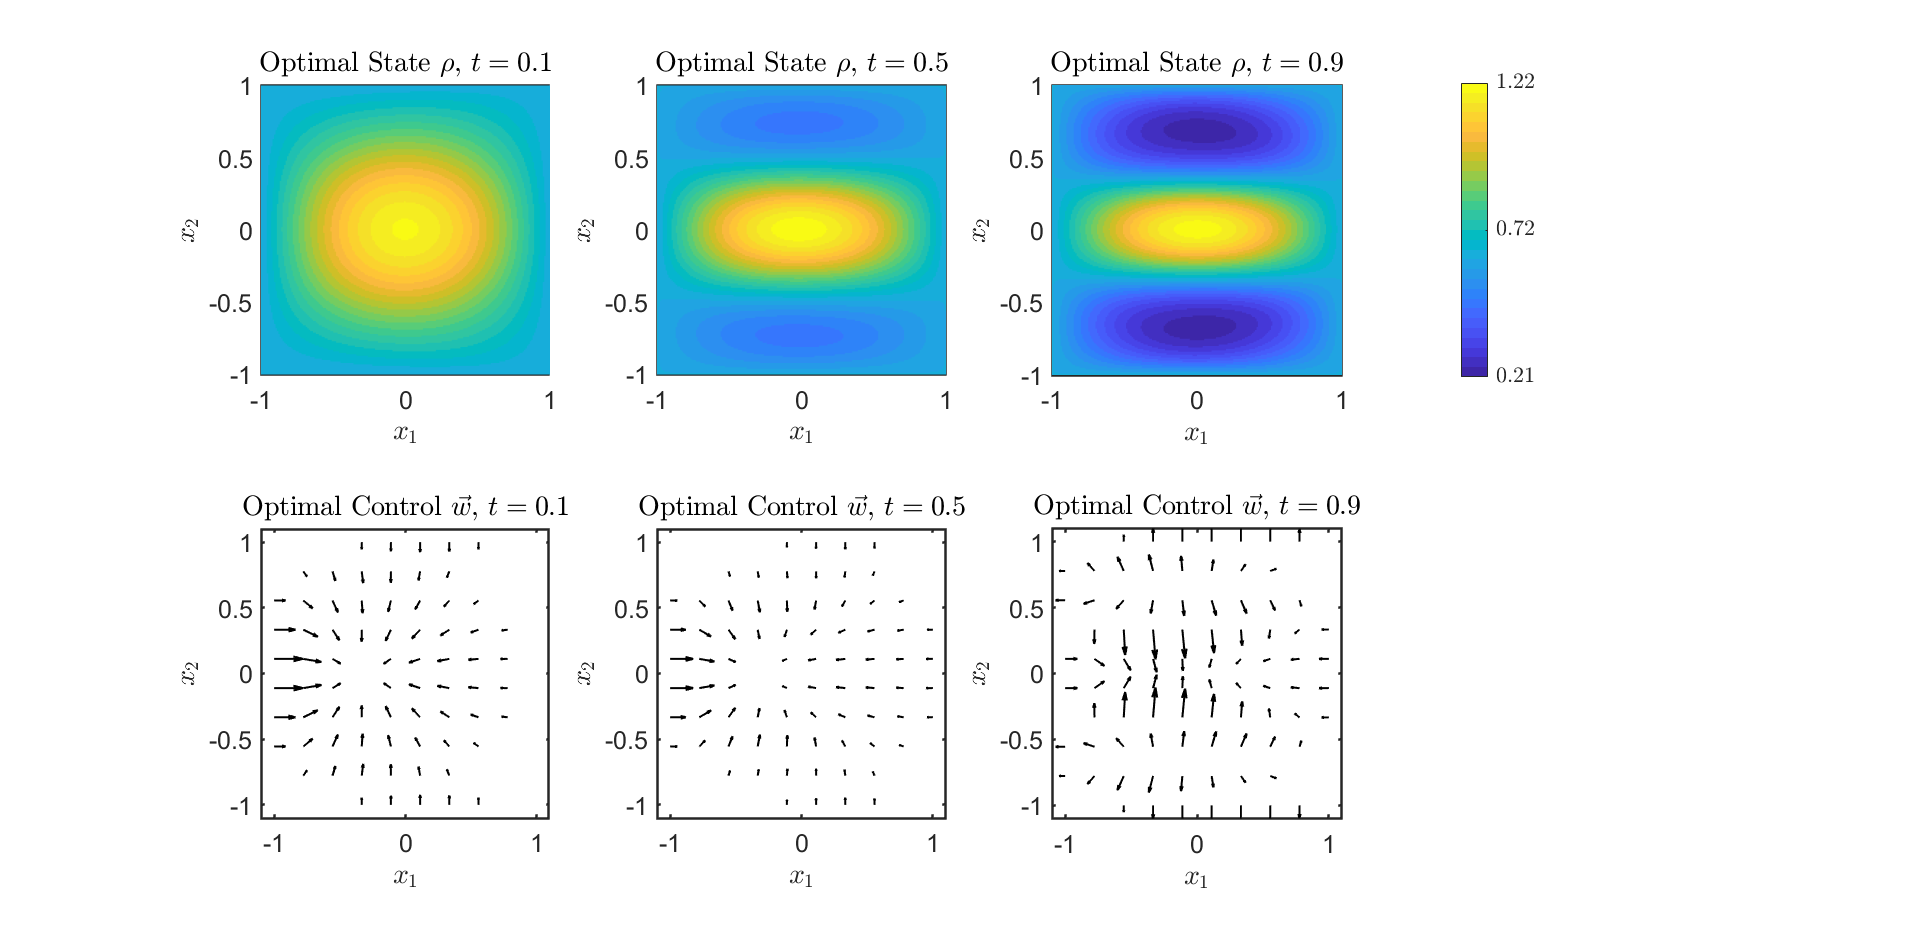
\includegraphics[scale=0.35]{FcEx2k1b.png}
		\caption{Dirichlet Flow Control 2: Optimal $\rho$ and optimal control for $\kappa = 1$ and $\beta = 10^{-3}$.} 
		\label{F5c}
	\end{figure}
	
\end{document}